In this chapter we present an evaluation of \name Baselines (See Chapter~\ref{sec:baselines}) in order to demonstrate how \name can extend the traditional hypothesis-based research, towards the Systematic Comparative Research approach we presented in Chapter~\ref{chap:problem-settings}. The content of this chapter is organised as follow:

In section~\ref{sec:experiment-design} we describe the method we use to design experiments for RSP Engine testing, and two test sets, SOAK Tests and Step Response Stress Tests. A complete description of the assumptions behind these two experimental sets can be found in Section~\ref{sec:soak-es} for the SOAK Test set and in Section~\ref{sec:step-es} for the Step Response one. 

With the SOAK Test set we aim of providing a simple use case with naive hypothesis, which highlights the limitations of the traditional top-down analysis approach applied to the SR research and which consequently demonstrates the fundamental role of \name  for RSP Engines evaluation.  The Step-Response tests are designed with the goal to show \name potential and to provide an alternative use case, which shows \name flexibility in supporting the Systematic Comparative Research Approach.

Finally, we present the experiment results respectively for SOAK test, in Section~\ref{sec:soakres}, and for the Step Response Test, in Section~\ref{sec:stressres}.

\section{Experiment Design}\label{sec:experiment-design}

Experiment design (ED) means defining our experiment in order to prove or refute one or more hypothesis, evidencing the behaviour of the system in a controlled execution environment. ED starts with some assumptions, which compose the  Experimental Setting. Researchers formulate hypothesis on the base of these assumptions, Figure~\ref{fig:experiment-design} summarises the collocation of ED within the Top-down approach.

\begin{figure}[tbh]
  \centering
	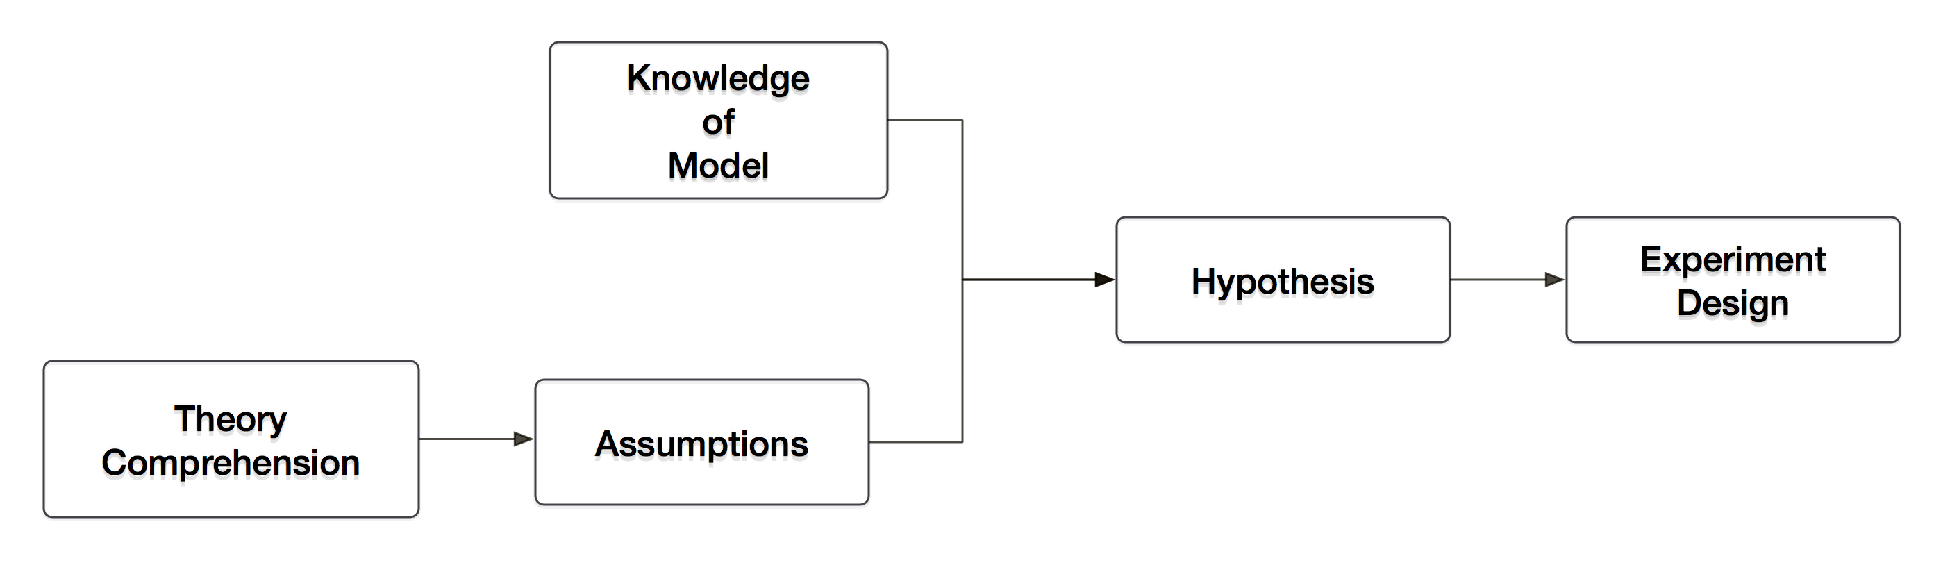
\includegraphics[width=\linewidth]{images/experiment-design}
	\caption[Experiment Design Process]{The traditional top-down research designs experiments in order to confirm or refuse hypothesis. The process starts from the theoretical knowledge, through which it is possible to formulate assumptions. Hypothesis are formulated observing an exiting model and considering the assumptions as known truths that simplify the environment. The design of a certain experiment depends on variations of the assumptions or on the variables involved.}
  	\label{fig:experiment-design}
\end{figure}

From a theoretical point of view we decide to study RSP Engine facing their nature of dynamic system. (see Section~\ref{sec:sfp}). Experiment design requires to point out which variable are observed. We simplify the study analysing their behaviour in term of Latency and Memory, which is, together with results completeness and soundness, the minimal meaningful measurement set for an RSP~Engine (Chapter~\ref{chap:heaven}).

In Chapter~\ref{chap:heaven}, we describe the experiment tuple: $<\mathcal{D}, \mathcal{T},\mathcal{E}, \mathcal{Q}>$ as:
\begin{itemize}
\item $\mathcal{E}$ is the RSP Engine
\item $\mathcal{D}$ is the Dataset 
\item $\mathcal{T}$ is the Ontology
\item $\mathcal{Q}$ is the Query that $\mathcal{E}$ continuously answers.
\end{itemize}

In this section we present our choices about the four elements that compose an experiment, upon which the evaluation is built.

\pagebreak

\subsection{Engine $\mathcal{E}$}

%. Top-Down investigations are commonly hard, and they become even harder for commercial solutions.
The architecture complexity of mature RSP Engines like the C-SPARQL Engine or CQELS is high, and it can not be easily faced in order formulate hypothesis of comparison. However, the purpose of this evaluation is showing how \name can improve the research of RSP Engine. Thus, we can simplify the research survey evaluating less complex systems. To this extent we design and implement the Baselines (Section~\ref{sec:baselines}) and we evaluate them as the RSP Engines $\mathcal{E}$ subject of our experiments. 

In Chapter~\ref{chap:problem-settings} we describe which requirements guarantee that an RSP Engine is a baselines: Simplicity, Elementarily, Relevance and Eligibility (SERE properties) legitimate the evaluation. Thus, the Baselines can be considered as a simple term of comparison for further research on Stream Reasoning systems and this investigation can be followed as a guideline.
 
The four baselines differ for two characteristics: RDF Stream Model and Reasoning architecture. The Table~\ref{tab:baselines-names} summarises these few but well determined differences, naming the four baselines for the evaluation:
\begin{table}[htb]
\centering
\normalsize
\begin{tabular}{c|cc} % creating eight columns
	\hline
         & Naive & Incremental\\
	\hline
	Graph        &  GN      & GI\\
	Triple   &  TN   & TI\\
	\hline % inserts single-
\end{tabular}
\caption[Baselines Naming Convention]{We name each baselines according to  the reasoning approach and the RDF Stream encoding. Thus an Incremental approach with a graph-based RDF Stream becomes GI.}
\label{tab:baselines-names}
\end{table}

\noindent Among these four configurations we can formulate simple hypothesis, stating which approach is better then an other one within an experiment. Notice that we have a complete model of the baseline systems and we also know many implementation details that can help during the analysis. We can exploit the know-how about their internal mechanisms, described in Section~\ref{sec:baselines-impl}, to lead our analysis from hypothesis formulation towards empirical results. 

\subsection{Dataset $\mathcal{D}$ and Ontology $\mathcal{T}$}\label{sec:dataset}

\noindent The Dataset  $\mathcal{D}$ and the Ontology $\mathcal{T}$ must be chosen to ensure baselines Simplicity, as stated in Section~\ref{sec:baselines}. 

The RDF Streams (see in Section~\ref{sec:rdfstream}) $\mathcal{D}$ used in the experiments are obtained streaming in different ways the data generated with LUBM (see Section~\ref{sec:lubm}). Consequently we chose LUBM ontology\footnote{http://swat.cse.lehigh.edu/onto/univ-bench.owl} as $\mathcal{T}$ for all the experiment. We assume that the ontology does not change over time, therefore the materialisation of $\mathcal{T}$ is computed before starting the experiment and the RSP engine does not have to perform this task. 

It is worth to discuss the choice of using data from LUBM rather than SRbench or LSbench. The first one has data, which are not adequate for the experiments, since they do not require any reasoning. The SRbench data, on the contrary, requires reasoning, but, being real-data, do not have the possibility to be scaled up and down. Further details on SRbench and LSBench can be found in Section~\ref{sec:lsbench}. Moreover, this choice is in line with previous works on Stream Reasoning~\cite{DBLP:conf/semweb/UrbaniMJHB13}. 

Being LUBM static data, we exploit the \textit{RDF2RDFStream} component of the \textsc{Test Stand} that takes care to adapt the data generate by LUBM to a streaming scenario (see Section~\ref{sec:streamer-impl}). \textit{RDF2RDFStream} is responsible to build $\mathcal{D}$ w.r.t. $\mathcal{T}$, scaling both in terms of dimension of the dataset and the reasoning effort. The component can be set up to obtain an RDF~Stream where the number of triples with the same timestamps follows a given distribution. %Section~\ref{sec:streamer-impl} contains all the details about the implementation and the usage of this particular \textsc{Streamer}. %e' veramente il timestamp quello?

\subsection{Query $\mathcal{Q}$}\label{sec:query}
 
The query $\mathcal{Q}$ used in our experiment depends on the reasoning approach of the RSP Engine in use. Actually, all  experiments uses variants of the same basic identity query that continuously asks for the materialisation of the active sliding window $\omega$, which differ from the sliding factor $\beta$.\\

\begin{center}
\raggedright
\small
REGISTER QUERY Q AS \\
SELECT ?s ?p ?o \\
FROM STREAM S [RANGE $\omega$ STEP $\beta$]\\
WHERE {?s ?p ?o}\\
UNDER $\rho$DF ENTAILMENT REGIME
\label{code:query}

\end{center}
Query:~\ref{code:query}: Query $\mathcal{Q}$ registered to the \name Baselines.\\


The Baseline GN and TN exploit the Naive Reasoning approach and thus the Query~\ref{code:query} is implemented in order to output the snapshot of the entire window at each slide of the window. On the other hand, the Baselines GI and TI exploit the Incremental Reasoning approach and thus they implement the Query~\ref{code:query} in order to output the ir-streams at each window slide.

The entailment regime of the RSP Engines influence performances. For this reason we take for the Baselines $\rho$DF, an RDF-S fragment that reduces complexity while preserving the normative semantics and core functionalities~\cite{DBLP:conf/esws/MunozPG07}. Several works in the field~\cite{DBLP:conf/semweb/UrbaniMJHB13, Liu:2014:ERS:2567948.2577323} choose $\rho$DF, because it is the minimal meaningful task for a Stream Reasoner.

\section{Experiment Set-Up}\label{sec:experiment-setup}

The \textit{RDF2RDFStream} allows to control the triple distribution in the RDF~Stream, thus it is possible to build experiment upon this distribution. 

We design set of SOAK Tests to evidence Baselines dynamics and, thus, evaluating their performances. 

In order to show \name potential, we design a small set of Stress Test, which belongs to the Step Response subcategory. In summary:

\begin{itemize}
\item \textbf{SOAK}: the number of contemporary triples in the RDF~Stream does not change during the experiment.
\item \textbf{Step Response} the number of contemporary triples in the RDF Stream does not changes for a certain period of time, which guarantees the system to reach a stable condition, then it suddenly increase or decrease. The number of triples in the RDF Stream does not changes any more, giving to the system the possibility to reach the stability again.
\end{itemize}

The queries registered to \name Baselines during all the experiments variate for the size of the sliding window $\omega$. In particular, we use windows in which $\omega$ is an integer multiple of the slide parameter $\beta$ of the window, i.e., it holds that $\omega = \beta * N$. In other words, $N$ is the number of \textsc{CTEvent}s that the window contain. 

Section~\ref{sec:baselines-impl} shows how the proposed baselines take advantage of the ability of Esper to be temporally controlled by an external agent\footnote{\url{http://esper.sourceforge.net/esper-0.7.5/doc/reference/en/html_single/index.html#api-controlling-time}} which sends time-keeping events to synchronise the internal time flow. All the triples in the \textit{CTEvent} are consider contemporary by the baselines and each \textit{CTEvent} can be seen as a proxy for the timing event. 

External time keeping and the \textit{RDF2RDFStream} make possible to estimate the content of the active window in terms of number of RDF Triples in any moment of the experiment.

All experiment are execute 10 times to reduce the presence of the outlier.

The following sections contain further details about the two test sets, respectively in Section~\ref{sec:soak-es} for SOAK Test and in Section~\ref{sec:step-es} for Step Response tests.

\subsection{SOAK: Tests and Hypothesis}\label{sec:soak-es}

SOAK testing show the system dynamics, injecting into the RSP Engine in use a constant and continuous input flow (see Section~\ref{sec:software-testing}). We maintain constant the number of contemporary triples in the RDF Stream through the \textit{RDF2RDFStream} module. %Moreover, Section~\ref{sec:query} describe how we variates the query between experiments.

SOAK Experiment are 30000 \textsc{CTEvent}s long. Each event contains a fixed number of RDF triples, which depends on the specific experiment. Unlikely, it is not possible to foretell how many events are required to reach the Steady State condition for each variable involved, especially memory. Multiple attempts and empirical evaluations are the only way to set up the correct duration.

\begin{table}[htb]
\centering
\small
 \begin{tabular}{l| ccccc}
	  	\hline
		\textsc{CTEvent}  &\multicolumn{5}{c}{Number of Slot}  \\
		Size  & 1 & 10 & 100 & 1000&10000 \\
		\hline	
		1 & 1& 10 & 100 & 1000&10000 \\
		10  & 10 & 100 & 1000&10000 \\
		100 & 100&1000&10000  \\
		1000 &1000 & 10000 \\
		10000&10000  \\
		\hline 
	\end{tabular}
	 \vspace{10pt}
	\caption[SOAK Tests Summary Table]{The number of triples in the window during the fifteen SOAK tests as a function of the window size (in terms of $N$) and of the triples in each \textsc{CTEvent}.}
	\label{tab:soaktests}
\end{table}

\begin{table}[htb]
	\centering
	\small
	\begin{tabular}{l | ccccc} % creating eight columns
	  	\hline
		Triple in & \multicolumn{5}{c}{Number of Slots}  \\
		Window  & 1 & 10 & 100 & 1000&10000\\
		\hline
		1  	 & 1\\
		10   & 10  & 1 \\
		100  & 100 & 10 & 1\\
		1000 & 1000& 100& 10& 1\\
		10000& 10000 & 1000& 100& 10& 1\\
		\hline % inserts single-line
	 \end{tabular}
	\caption[SOAK Tests Summary Table Alternative Layout]{The number of triples in a \textsc{CTEvent} during the fifteen SOAK tests as a function of the window size (in terms of $N$) and of the total triples in the active window, assuming one and only one \textsc{CTEvent} per slot.}
	\label{tab:soaktests-alt}
\end{table}

Table~\ref{tab:soaktests} presents the fifteen SOAK tests we run for. The columns of the table are the different window sizes measured in terms of the values assumed by the number of slots $N$ (see Section~\ref{sec:query}).  Being $\beta=$ 100 ms., they correspond to a window that spans 100 ms., 1 sec., 10 sec. and 100 sec.. The rows are the different number of triples in each \textit{CTEvent} sent by the \textsc{RDF2RDFStream} to $\mathcal{E}$.% Notably, for all of them, we checked that $\mathcal{E}$ is responsive for the whole duration of the experiment. 

Table~\ref{tab:soaktests-alt} is an alternative layout where the columns of the table still contain the different window sizes measured in terms of the values assumed by the number of slots $N$, while the rows are the different number of triples in the active window. This layout allows to highlight the window dimension, focusing on the element which actually influences the reasoning.\\

\noindent Following the traditional research method, we formulate two naive hypothesis based on the knowledge we have of the easiest RSP Engine model (detailed in Section~\ref{sec:baselines}). 

From theory we know that the incremental maintenance of the materialisation is more convenient when the dimension of the changes is small w.r.t the entire window, otherwise  for large changes it is more computationally expensive than naive materialisation~\cite{DellAglio2014,DBLP:conf/cikm/RenP11,DBLP:conf/semweb/UrbaniMJHB13}.
This knowledge allow us to formulate a first hypothesis, which can state that the incremental reasoning approach is always better than the naive one, for small changes i.e. we consider small changes equal or less 20\% of the active window content.

From recent works like~\cite{DBLP:conf/semweb/BalduiniVDTPC13} we know that the graph data structure may speed up reasoning when it contains multiple triples, but it does so introducing an overhead that may hinder performances when it contains few triples. Thus, we can formulate a second hypothesis, which affirms that the triple-based model for RDF Stream is always better than the graph-based one when the number of triples in the graphs is small, i.e 20\% of the active window.\\

More formally the hypothesis to verify with SOAK experiments are:
\begin{itemize}
\item \textbf{HP.1} The Incremental reasoning approach is always better than the naive one for small changes.
\item \textbf{HP.2} The Triple-based model for RDFStream is always better than the Graph-based one if we consider few triples, to compose each graph.
\end{itemize}

%Notice that the goal of this evaluation is to show how \name helps RSP Engine analysis through empirical research. Hypothesis verification and top-down analysis are the subject of our investigation, while our research question is:  "\textit{Can an engine test stands, together with queries, datasets and methods, support Systematic Comparative Research Approach for Stream Reasoning?}" %"Needs the Stream Reasoning research field a Test Stand like \name to investigate RSP Engines and sustain the research of such system with an Systematic Comparative Approach?"

\subsection{Step Response Tests}\label{sec:step-es}

Step Response testing allows to see how the system reacts to a sudden changing in the input condition (see Section~\ref{sec:software-testing}). They are related to SOAK test, because they allow to study deeply the initial warm-up phase of the system. This set of experiments evidences the different responses of an RSP Engine if we move from an input condition to another instead of starting from scratch.

Step Response experiments are 40000 \textsc{CTEvent}s long. Since this duration requires hours of execution we investigate only few configurations, all with a slots number of 10. Table~\ref{tab:steptests} summarises the step experiment set-up, where the step is positioned at the half of the execution, 20000 events.
\begin{table}[htb]
\centering
 \begin{tabular}{c|c|c}
	  	\hline
	  	&\multicolumn{2}{c}{CTEvent size}  \\
		Number of Slots & Initial Size & Final Size\\
		\hline
		\hline
		 10 & 10 & 100\\
		 10 & 100 & 1000\\
		 10 & 10 & 1000\\
		\hline 
 \end{tabular}
 \caption[Step Response Tests Summary Table]{Step Response Test Summary Table -  the first column indicates that every Step Response test is executed with a number of slot equals to 10. At the beginning of the experiment the \textsc{CTEvent} sizes are indicated in the second column, while their sizes at the end of the experiment is reported in the third and last column. All the Step Response tests are 40.000 \textsc{CTEvent}s long, and the step position is always at the half of the experiment duration, thus 20.000 \textsc{CTEvent}s}
\label{tab:steptests}
\end{table}

We do not formulate hypothesis for Step experiments. The purpose of this test set is to show \name potential in term of analysis an experiment design. They shows how it is possible to set up \name in order to stress an RSP Engine in many ways.

\subsection{Execution Environment}\label{sec:execution-environment}

Before presenting experiment results, a brief description of the execution environment is required. All experiment are executed exploiting a dedicated machine, an iMac mid-2011 with 12GB RAM and 3.6 Ghz of a Intel i5 64 Bit, which run OS X 10.10.2 Yosemite,. Since \name is developed with Java 7\footnote{http://www.oracle.com/technetwork/java/javase/javase7locales-334809.html}, we use the versione 1.7.0.71 of the JVM.
The execution happens in a controlled environment, which tries to reduce the number of disturbing elements like network, graphical interface and other running processes.

\section{SOAK Test Evaluation Results}\label{sec:soakres}

In this section, we analyse the results of the SOAK Test experiments, exploiting the investigation stack presented in Chapter~\ref{chap:heaven}. The analysis goes through the four levels of the stack, with the aim of confirming or refusing the hypothesis presented in Section~\ref{sec:soak-es}. 

The content of this section is organised as follow: 
Section~\ref{sec:eval-ssib} presents the output of the \textit{Steady State Identification} block. 
Section~\ref{sec:eval-level0} presents the results obtained at Level 0, the dashboard visualisation.  
Section~\ref{sec:eval-level1} provides a qualitative comparison for latency and memory, built at Level 1. 
Section~\ref{sec:eval-level2} contains example of pattern identification at Level 2. 
Finally, in Section~\ref{sec:eval-level3}, we include some examples of the Level 3 \textit{Intra Experiment }comparisons, while in Section~\ref{sec:stressres} we include examples of \textit{Inter Experiment }ones w.r.t the Step Response tests.


\subsection{Steady State Identification Block Results}\label{sec:eval-ssib}

The \textit{Steady State Identification} (SSI) block, as reported in Chapter~\ref{chap:implementation-experience}, annotates the averaged raw data received by the \textit{Pre-Processing} block, indicating which variable has reached a Steady State condition for an experiment. Table~\ref{tab:ss-cond} contains all the results the SSI Block, distinguishing between latency and memory for each variables


\begin{table}[htb]
\centering
\scriptsize
 \begin{tabular}{c|c|c|cc|cc|cc|cc}
	  	\hline
	  	&&&\multicolumn{8}{c}{Steady State Condition Identification Result}  \\
	  	&CTEvent&&\multicolumn{2}{c}{GN}|&\multicolumn{2}{c}{GI}|&\multicolumn{2}{c}{TN}|&\multicolumn{2}{c}{TI}  \\
	  	EN&Size& Slot Num.&Lat&Mem&Lat&Mem&Lat&Mem&Lat&Mem  \\
		\hline
		\hline
		 1&1&1&Yes&Yes&Yes&No&Yes&Yes&Yes&Yes\\
		 2&10&1&Yes&Yes&Yes&Yes&Yes&Yes&Yes&Yes\\
		 3&100&1&Yes&Yes&Yes&Yes&Yes&Yes&Yes&Yes\\
		 4&1000&1&Yes&Yes&Yes&Yes&Yes&Yes&Yes&Yes\\
		 5&10000&1&NA&NA&NA&NA&NA&NA&NA&NA\\
		 6&1&10&Yes&Yes&Yes&Yes&Yes&Yes&Yes&Yes\\
		 7&10&10&Yes&Yes&Yes&Yes&Yes&Yes&Yes&Yes\\
		 8&100&10&Yes&No&Yes&No&Yes&No&Yes&No\\
		 9&1000&10&Yes&Yes&Yes&Yes&Yes&Yes&Yes&Yes\\
		 10&1&100&Yes&No&Yes&Yes&Yes&Yes&Yes&Yes\\
		 11&10&100&Yes&No&Yes&No&Yes&No&Yes&No\\
		 12&100&100&Yes&Yes&Yes&Yes&Yes&Yes&Yes&Yes\\
		 13&1&1000&Yes&No&Yes&No&Yes&No&Yes&No\\
		 14&10&1000&Yes&Yes&Yes&Yes&Yes&Yes&Yes&Yes\\
		 15&1&10000&Yes&Yes&Yes&Yes&Yes&Yes&Yes&Yes\\

		\hline 
 \end{tabular}
 \caption[Steady State Identification Block - Output Summary Table]{Steady State Identification Block - Output Summary Table - Experiment number follows the layout of Table \ref{tab:soaktests-alt}, filling the columns from the top to the bottom. The Steady State condition is evaluated after the average value of  25.000 \textsc{CTEvent}s,  corresponding to the 85\% of the experiment duration. Despite it is an excessive quantity for the latency Steady State evaluation, even in case of filling phenomena, it is not enough for the memory evaluation of several experiments.}
 \label{tab:ss-cond}
\end{table}

All the SOAK Experiments reach the Steady State condition for latency, but some of them did not for memory. Notice in particular that GI does not reach the memory Steady State for experiment 1 (  \textsc{CTEvent}  Size = 1000 and a number of slot = 1). Moreover, all the baselines do no reach the memory  Steady State for experiments 8, 11, 13, ( \textsc{CTEvent}  Size = 1000 and a number of slot from 10 to 1000). 

Experiment number 5 ( the \textsc{CTEvent} Size = 10000 a slot Nnumber = 1=) did not terminate correctly for all the baselines, due to an execution error and thus, its results are not part of our evaluation.

\subsection{Level 0 - Dashboard Views}\label{sec:eval-level0}

\begin{figure}[htb]
	\centering
	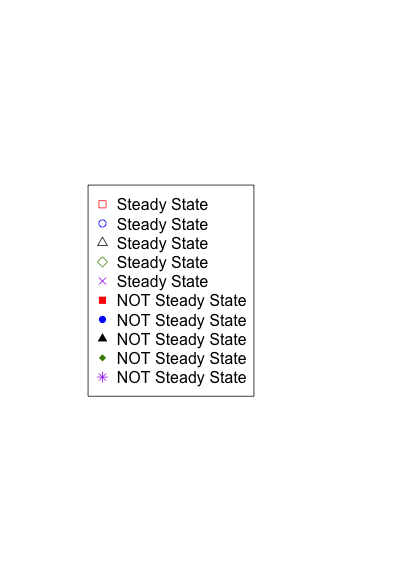
\includegraphics[width=0.25\linewidth]{images/dashboard-legend}	
	\caption{Dashboard Legend} 
	\label{fig:dashboard-legend}
\end{figure}

The SOAK test results analysis starts with the dashboard view at Level 0. Each dashboard presented is composed by two charts which shows in different from the relation between the different four baselines.  Figure~\ref{fig:dashboard-legend} shows the dashboard legend, which is fixed for all the charts related to the SOAK tests.

\subsubsection{Dashboard One - Fixed Size \textsc{CTEvent} = 1} 

\begin{figure}[h!tb]
	\centering
	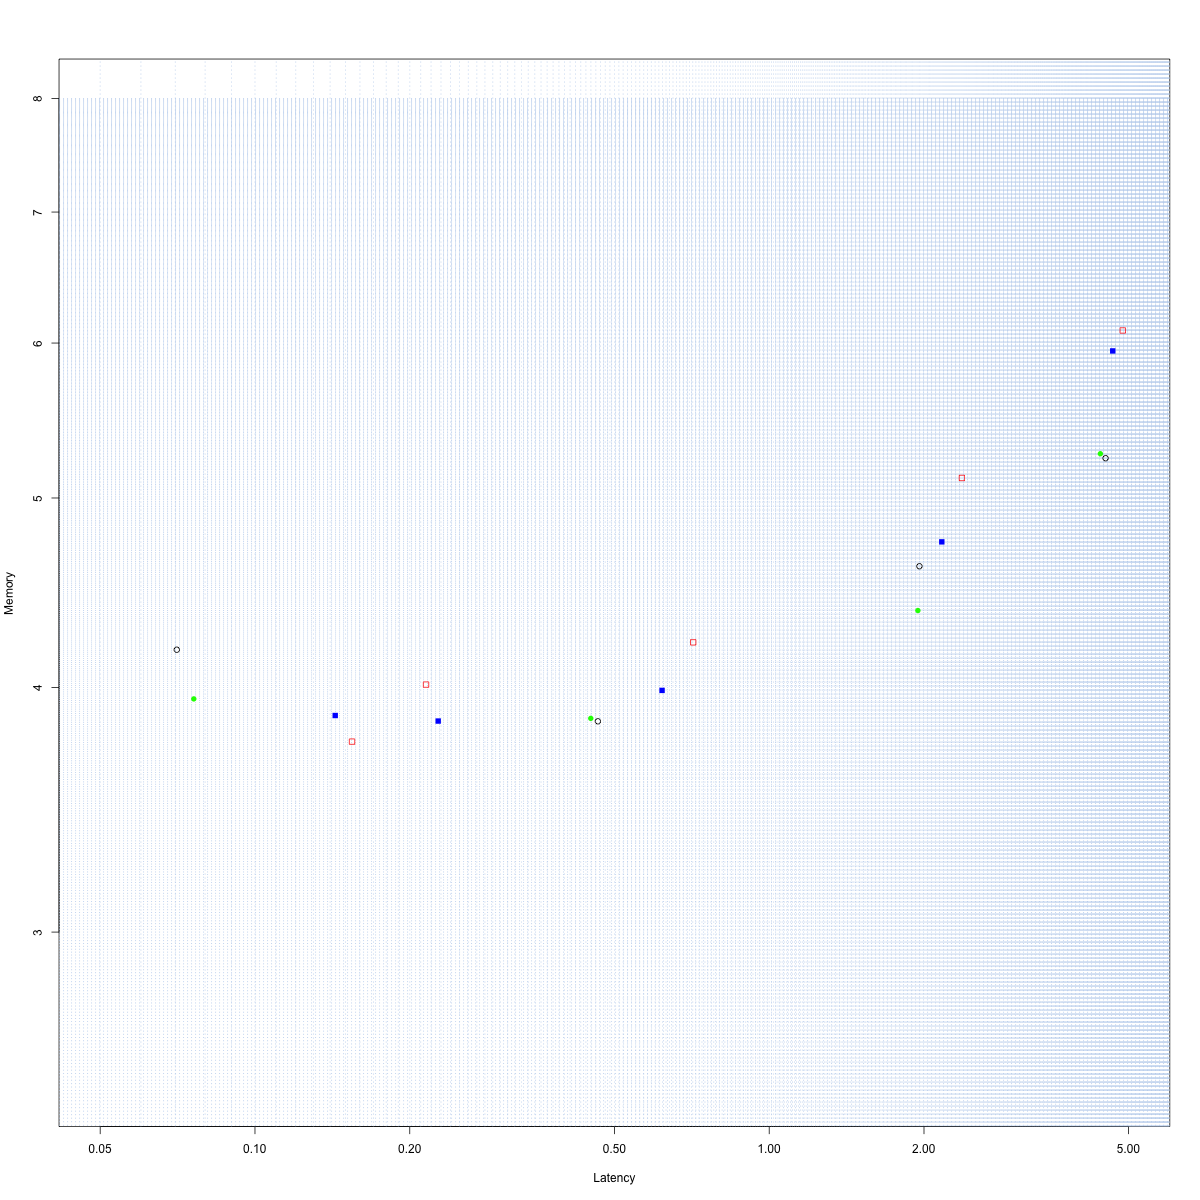
\includegraphics[width=0.85\linewidth]{images/dashboard-1}	
	\caption[\textsc{Analyser} Investigation Stack - Level 0 - Dashboard One - Multiplot Version]{\textsc{Analyser} Investigation Stack - Level 0 - Dashboard One - The figure shows how the Baselines performances (avg memory (y) and latency (x)) variate between a subset of SOAK Test experiments, composed by experiments with a constant \textsc{CTEvent} Size (K) = 1 triple (Experiment (EN) 1,6,10,13,15).} %EW indicates the number of slots in the window.} 
	\label{fig:result_dashboard_kb}
\end{figure}

\begin{figure}[t!hb]
	\centering
	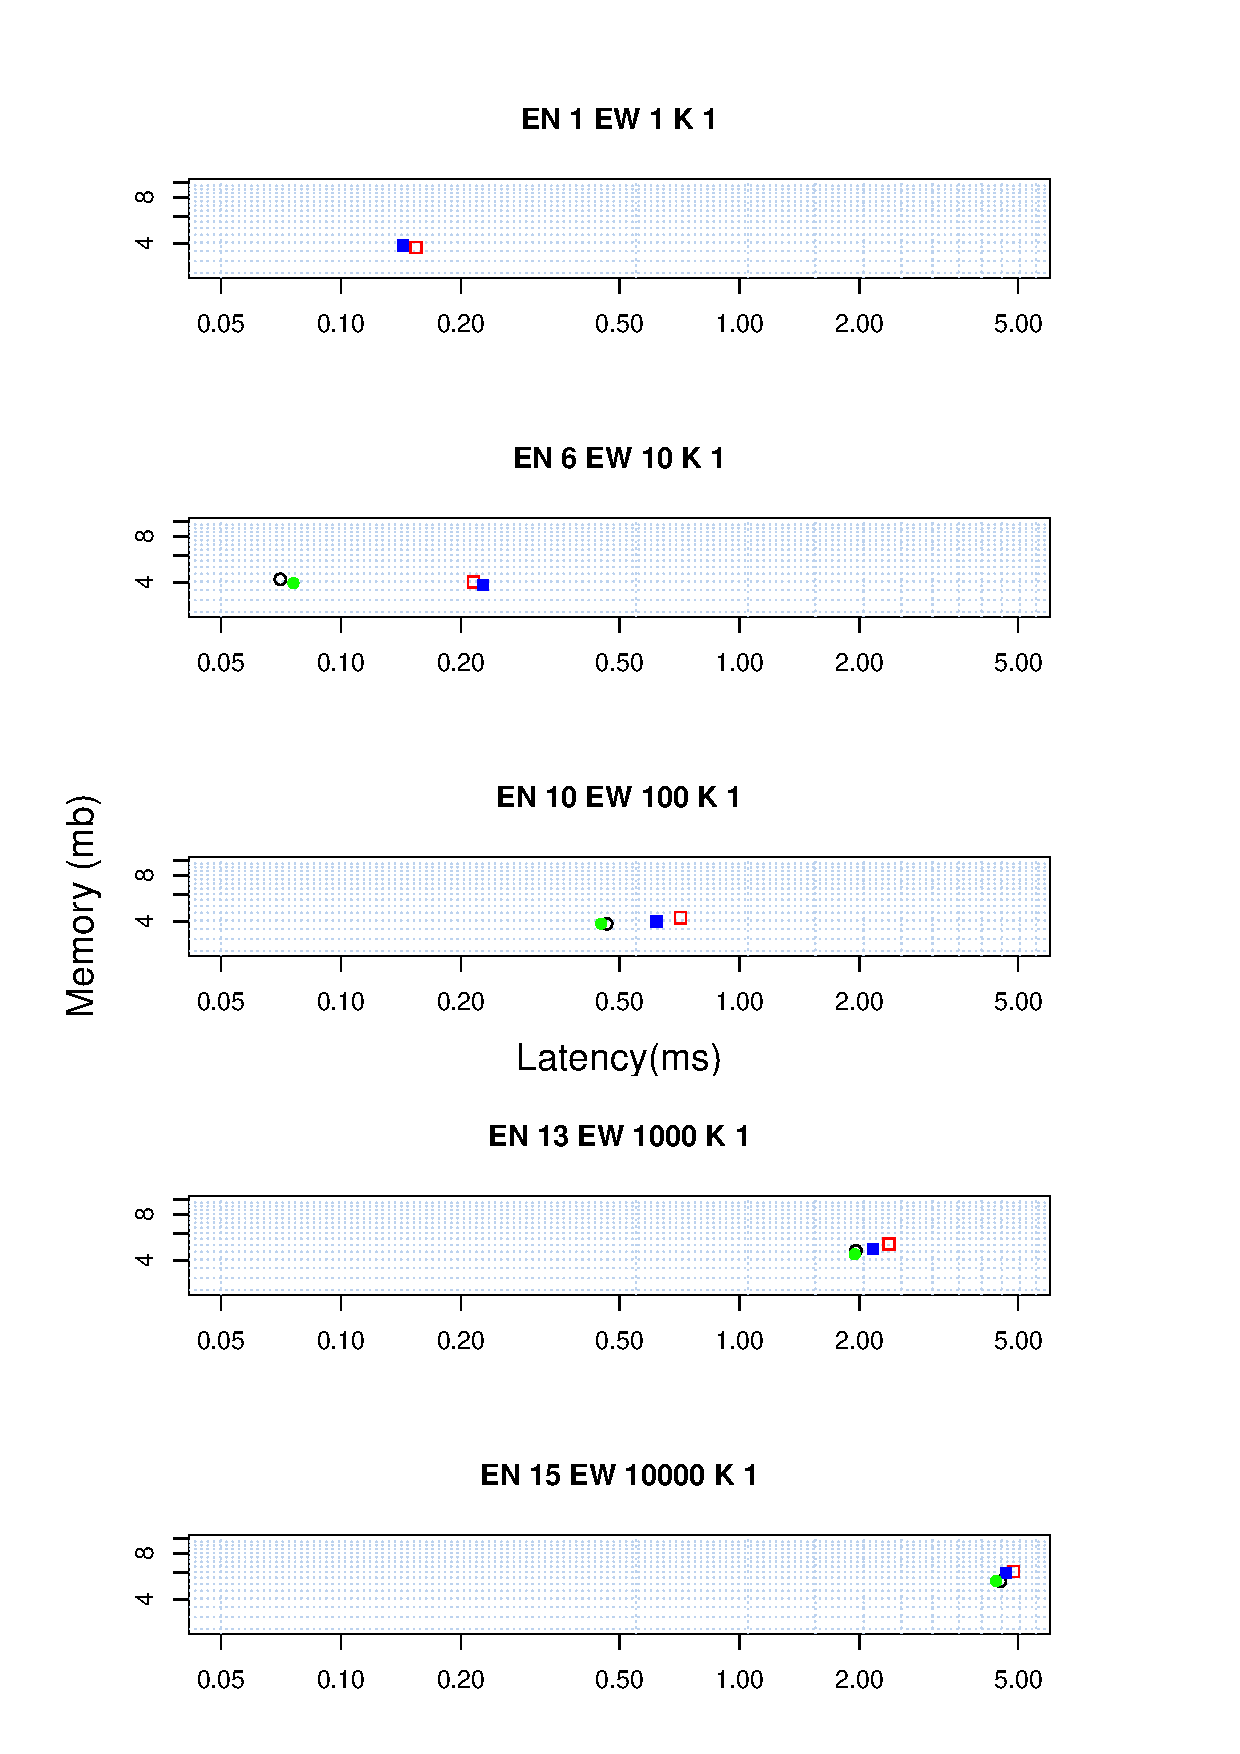
\includegraphics[width=\linewidth]{images/dashboard-1-split}	
	\caption[\textsc{Analyser} Investigation Stack - Level 0 - Dashboard One - Split Version]{\textsc{Analyser} Investigation Stack - Level 0 - Dashboard One - The figure shows how the Baselines performances (average memory (y) and latency (x))  variate between a subset of SOAK Test experiments, composed by experiments with a constant \textsc{CTEvent} Size (K) = 1 triple (Experiment (EN) 1,6,10,13,15); EW indicates the number of slots in the window. The results are reported comparing experiments on different stand alone plots.} 
	\label{fig:result_dashboard_ka}
\end{figure}

Figures~\ref{fig:result_dashboard_ka} shows how the behaviour of the four Baselines changes between a set of experiments which has a fixed CTEvent size of 1 triple and variates the number of slot in the active window, from 1 (Tumbling) to 10000. This configuration means moving on the latest diagonal of Table~\ref{tab:soaktests-alt}.

In Figure~\ref{fig:result_dashboard_ka}, we can appreciate that increasing the number of slots in the active window, and thus the window size in terms of triple, all the baselines show latency worsening. The Baselines which exploits the Incremental reasoning approach, GI and TI, are not represented in the figure when the number of slides is equal to one (Tumbling window of only one triple), because their latency it too small to be represented in this scale. Increasing the number of slot, GI and TI have the bigger worsening in term of latency than GN and TN. Actually, they do not became worse, but the Incremental approach is at least comparable with the naive one, when the number of slots became high (10000) and the variation is about 2/10000.

Observing Figure~\ref{fig:result_dashboard_kb}, which shows all the experiment within a single image, we can also individuate the worsening for the memory consumption. A first obvious insight may be that \textit{Bigger problem requires in general more resources}. %Another insight regards the difference in term of latency, the x-asis, between the different baselines.

Dashboard One confirms Hypothesis [Hp.1], the incremental approach performs better than the naive one for both latency and memory, and it partially confirms  [Hp.2]: the latest results in Figure~\ref{fig:result_dashboard_ka} shows that the memory usage depends on the reasoning approach and thus the relation between graph-based streams and triple-based one depends on it too. The figure confirms [Hp.2], the latency is smaller in experiments with a big window and a triple-based stream, while for smaller windows a graph-based one may work better.


\subsubsection{Dashboard Two - Fixed Number of Slot = 10}


\begin{figure}[h!tbp]
	\centering
	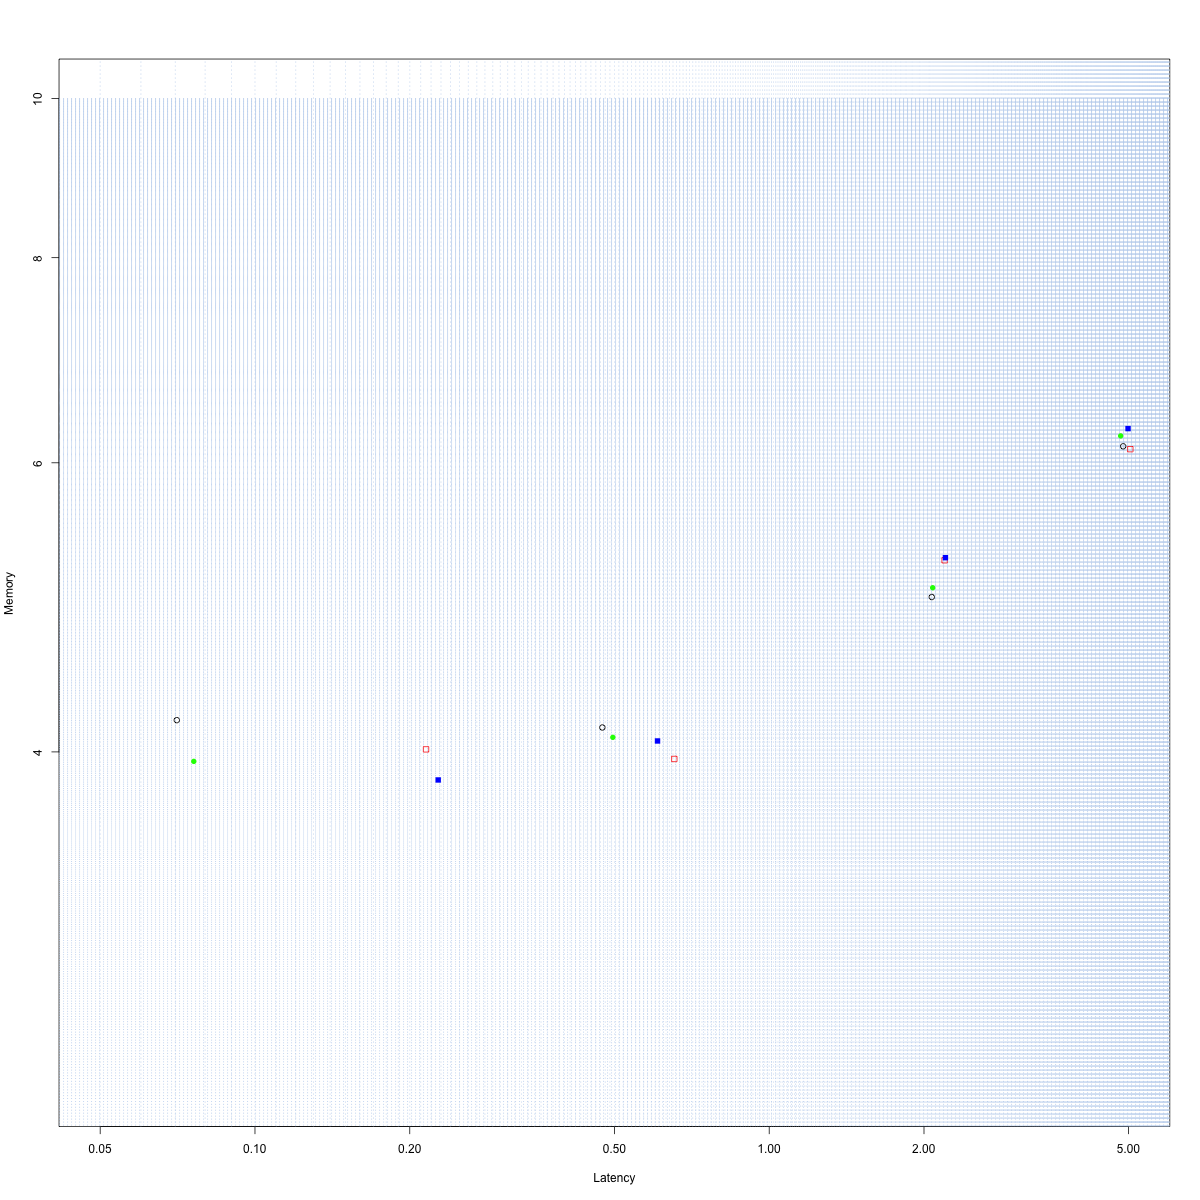
\includegraphics[width=0.85\linewidth]{images/dashboard-2}	
	\caption[\textsc{Analyser} Investigation Stack - Level 0 - Dashboard Two - Multiplot Version]{\textsc{Analyser} Investigation Stack - Level 0 - Dashboard Two - The figure shows how the Baselines performances (average memory (y) and latency (x)) variate between a subset of SOAK Test experiments, composed by experiments with a constant number of slots in window (EW) of 10 (Experiment (EN) 6,2,8,9).} 	% K indicates the \textsc{CTEvent} size.
	
	\label{fig:result_dashboard_ewb}
\end{figure}

\begin{figure}[h|tbp]
	\centering
	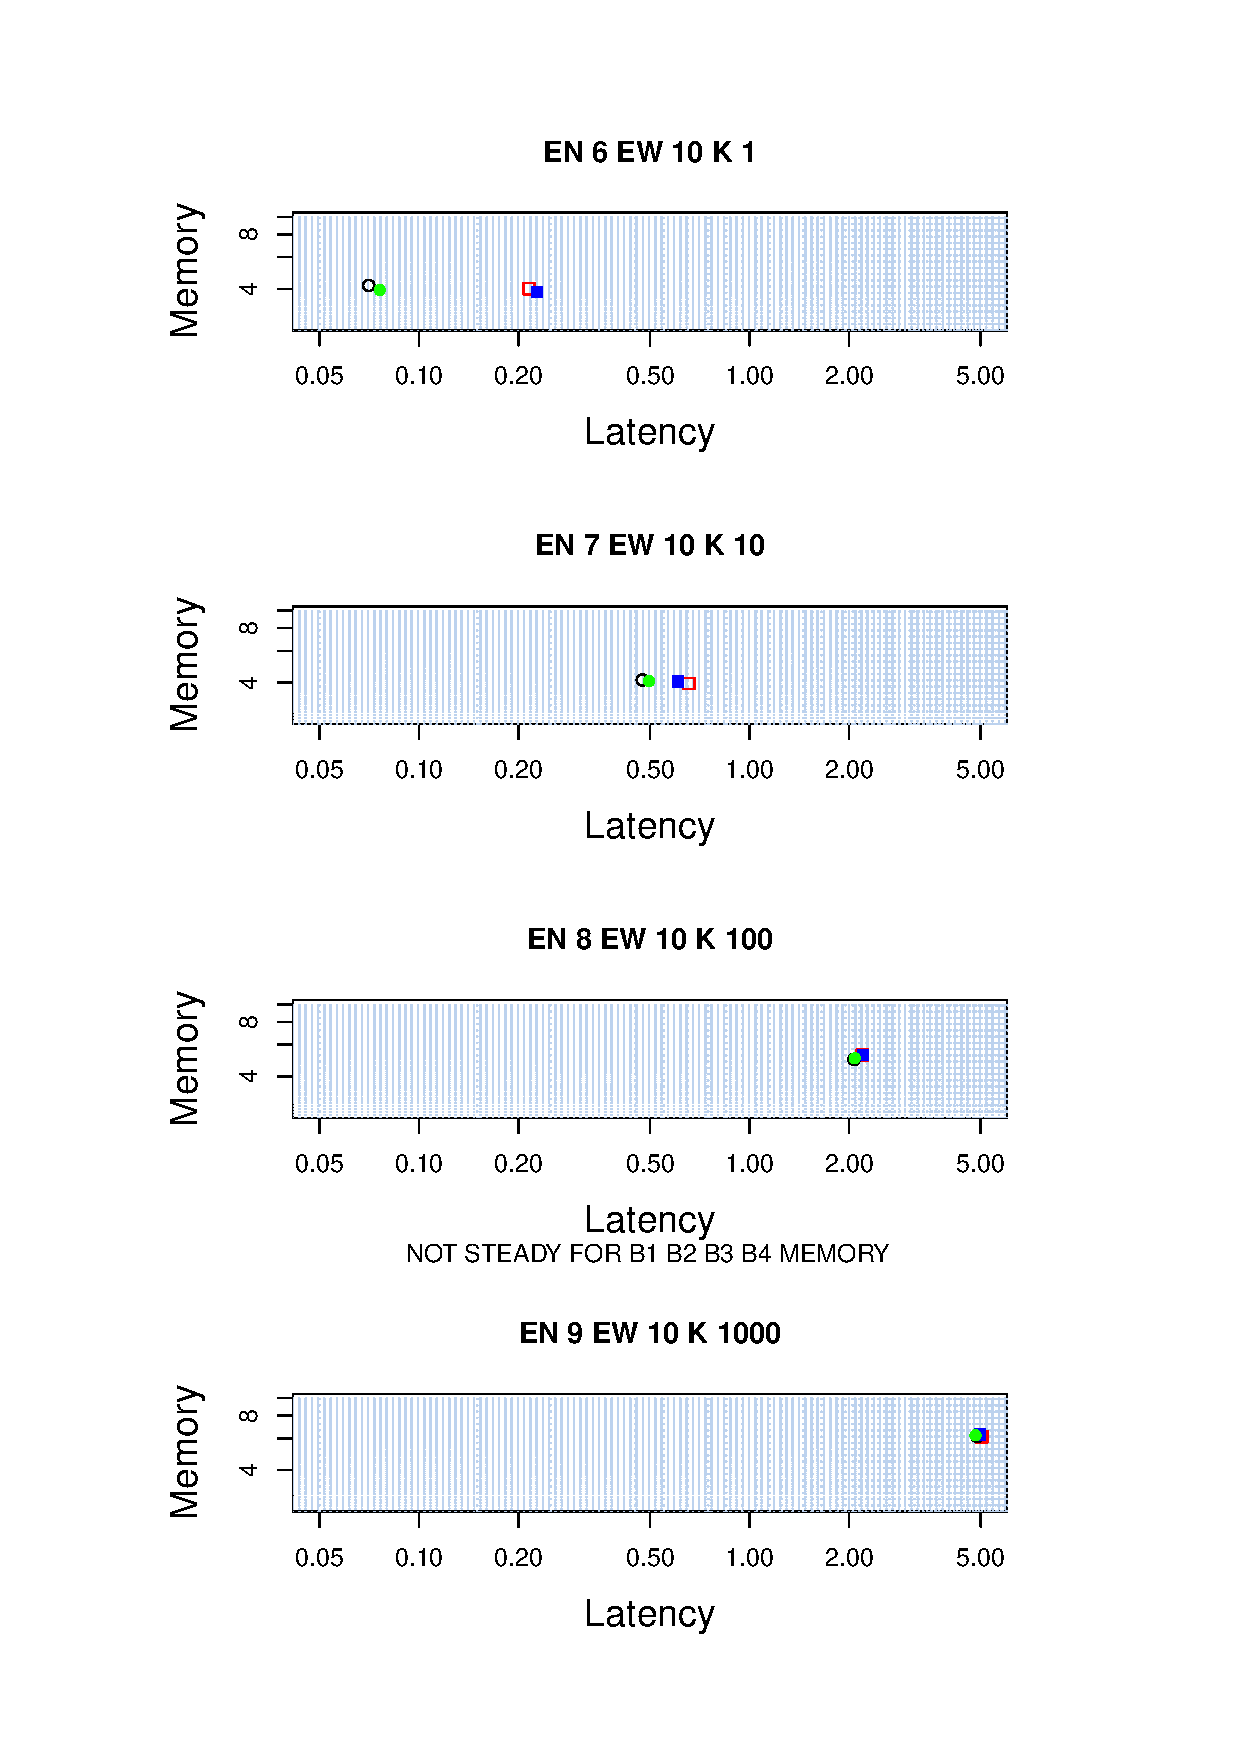
\includegraphics[width=0.80\linewidth]{images/dashboard-2-split}	
	\caption[\textsc{Analyser} Investigation Stack - Level 0 - Dashboard Two - Split Version]{\textsc{Analyser} Investigation Stack - Level 0 - Dashboard Two - The figure shows how the Baselines performances (average memory (y) and latency (x))  variate between a subset of SOAK Test experiments, composed by experiments with a constant number of slot in window (EW) of 10 (Experiment (EN) 6,2,8,9). K indicates the \textsc{CTEvent} size. The results are reported comparing experiments on different stand alone plots.}
	\label{fig:result_dashboard_ewa}
\end{figure}

Figure~\ref{fig:result_dashboard_ewa} shows how the behaviour of the four Baselines changes between a set of experiments which have a fixed number of 10 slots in the active window, while the size of the \textsc{CTEvent} changes from 1 to 10000. This analysis means, w.r.t Table~\ref{tab:soaktests-alt} layout, moving from the top to the bottom of the second column.

From the observation of the two figures emerges that: (1) Latency worsening is still clearly visible in Figure~\ref{fig:result_dashboard_ewa}, while the memory ones requires Figure~\ref{fig:result_dashboard_ewb}; (2) The behaviour of the baselines becomes indistinguishable when the window size in terms of triple is grown too much. 

[Hp.1] is confirmed for the latency performance, as can be seen in Figure~\ref{fig:result_dashboard_ewb}, GN and TN are always slower than GI and TI. 

For memory, the results are ambiguous and requires further investigations, only 50\% of the experiments confirm the hypothesis. Figure~\ref{fig:result_dashboard_ewb} shows that [Hp.2] is confirmed within a single reasoning approach, while in general the results are similar to the ones of [Hp.1].

\subsubsection{Dashboard Three - Fixed Windows Size (Triples) = 10000 } 

\begin{figure}[h!tbp]
	\centering
	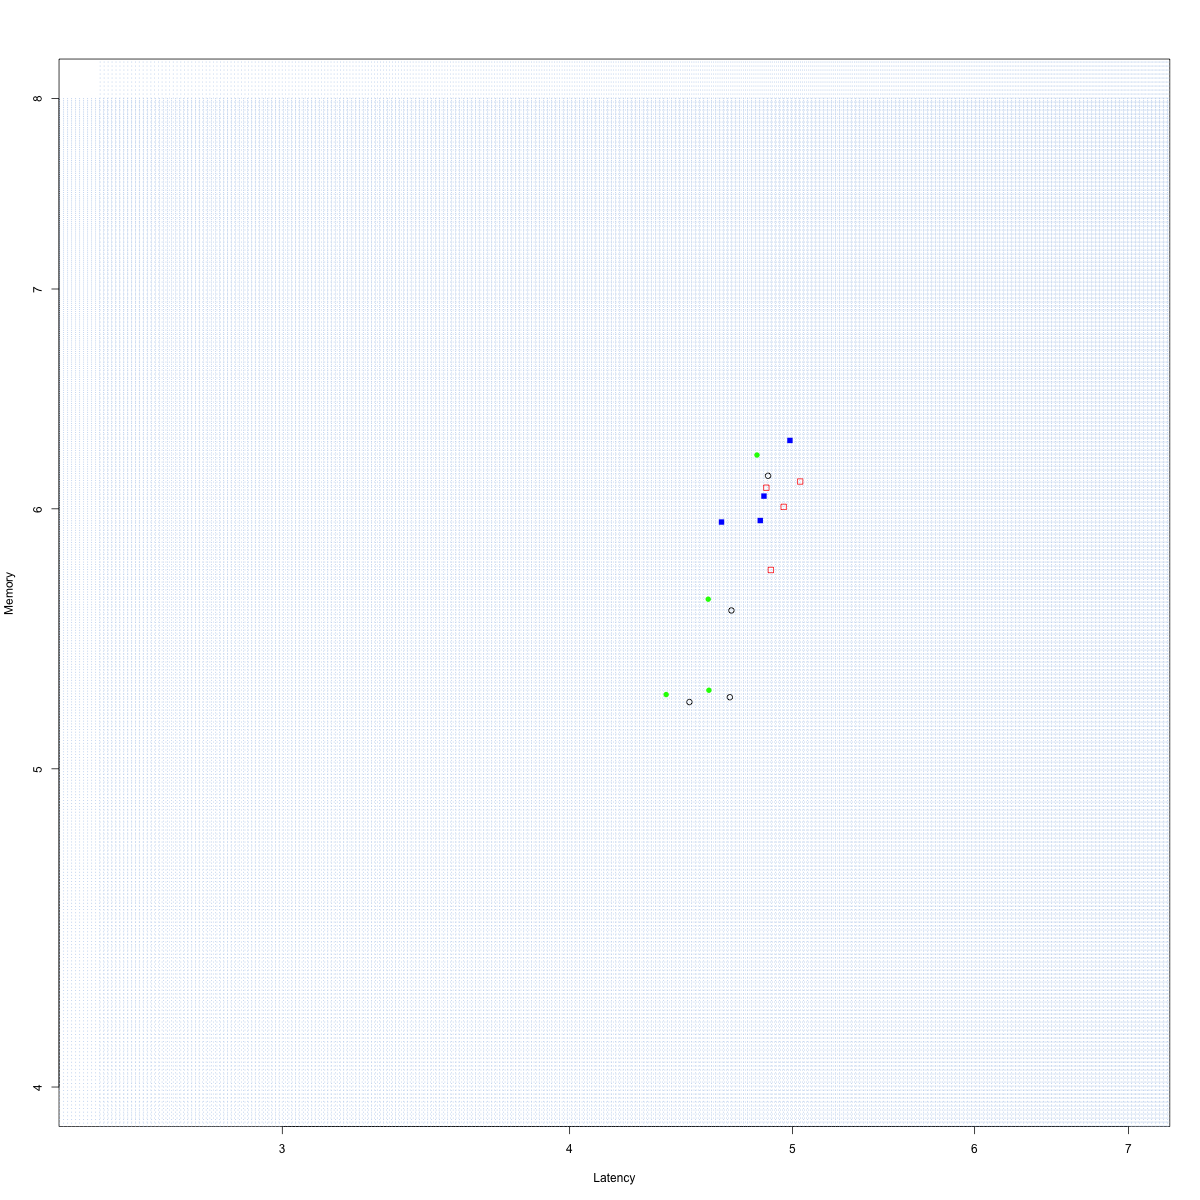
\includegraphics[width=0.85\linewidth]{images/dashboard-3}	
	\caption[\textsc{Analyser} Investigation Stack - Level 0 - Dashboard Three - Multiplot Version]	{\textsc{Analyser} Investigation Stack - Level 0 - Dashboard Three - The figure shows how the Baselines performances (average memory (y) and latency (x))  variate between a subset of SOAK Test experiments, composed by experiments with a constant number of triple in the active window, thus a constant product of \textsc{CTEvent} Size (K) * Num.Slots (EW) = 10000 (Experiment (EN) 9,12,14,15, experiment 5 is excluded for an erroneous execution).}
	\label{fig:result_dashboard_probb}
\end{figure}

\begin{figure}[h!tbp]
	\centering
	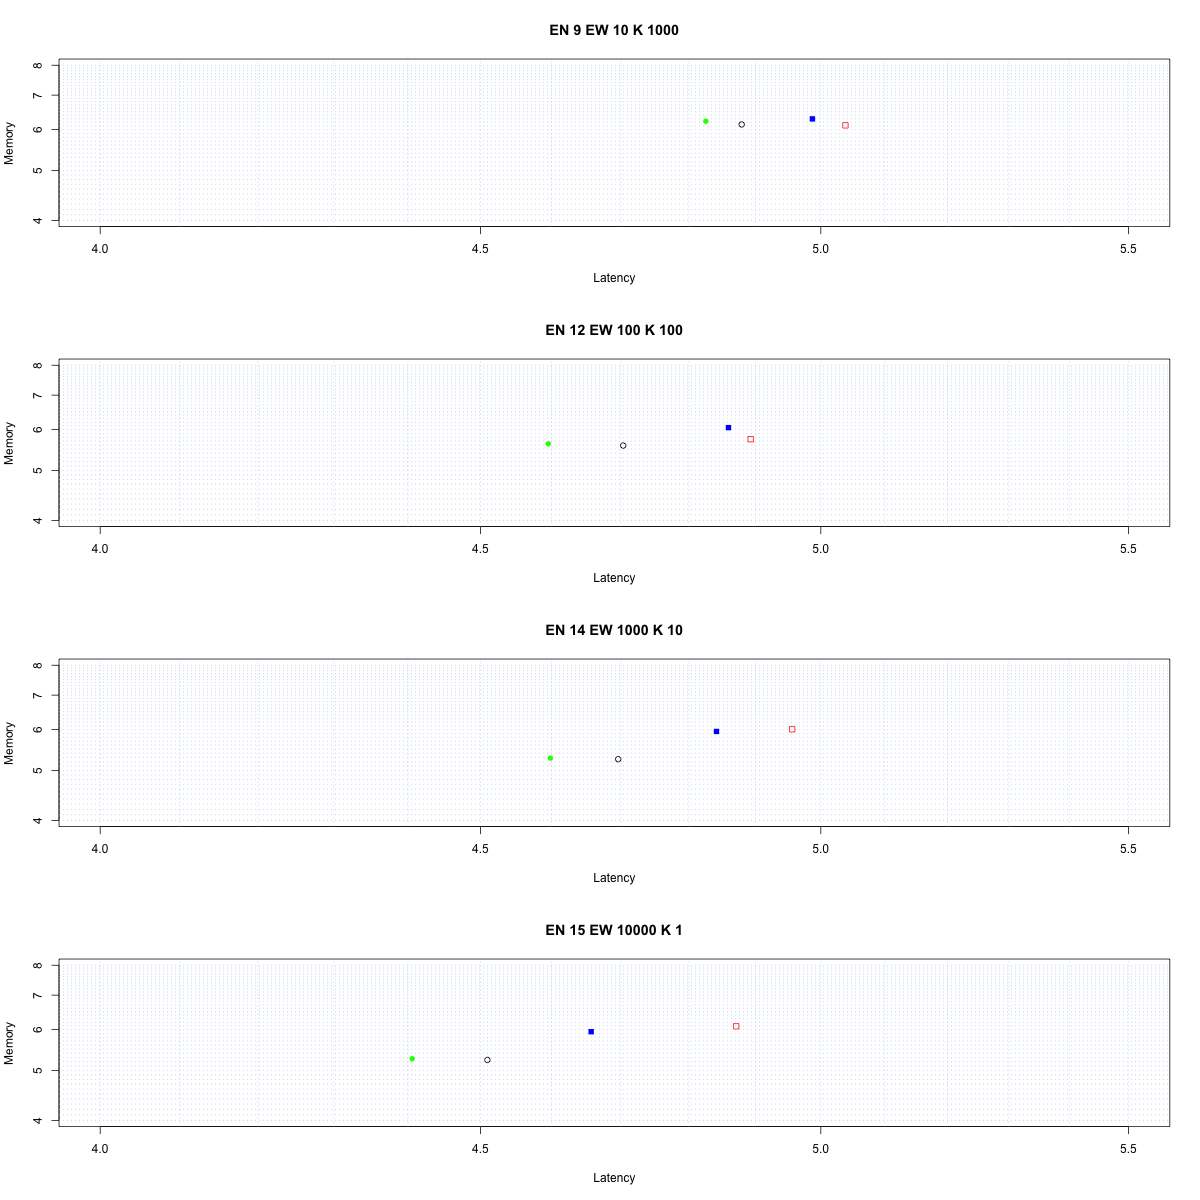
\includegraphics[width=0.75\linewidth]{images/dashboard-3-split}	
	\caption[\textsc{Analyser} Investigation Stack - Level 0 - Dashboard Three - Split Version]	{\textsc{Analyser} Investigation Stack - Level 0 - Dashboard Three - The figure shows how the Baselines performances (average memory (y) and latency (x)) variate between a subset of SOAK Test experiments, composed by experiments with a constant product of \textsc{CTEvent} Size (K) * Num.Slots (EW) = 10000 (Experiment (EN) 9,12,14,15 - 5 is excluded for an erroneous execution).  The results are reported comparing experiments on different stand alone plots.}
	\label{fig:result_dashboard_proba}
\end{figure}

Figure~\ref{fig:result_dashboard_proba}  shows how the behaviour of the four Baselines changes between a set of experiments which have a constant number triples within the active window equal to 10000, stated by maintaining the product \textsc{CTEvent} size (K) and Slot Number (EW) constant to 10000 triples. Fixing the window size in terms of triple to 10000 means moving from the left to the right on the lowest row of Table~\ref{tab:soaktests-alt}. 

The main observation we can state on Figures~\ref{fig:result_dashboard_proba} and~\ref{fig:result_dashboard_probb}  is that the baselines performances seems depending only on the dimension of the active windows, indeed for all the observed experiment  baselines memory usage and latency are disposed in a small interval.

[Hp.1] is confirmed for both the memory and the latency as the figures show. However the difference are very small between the approaches. [Hp.2] is confirmed again observing a single reasoning approach at time, while in general it is not possible to say that Triple-based RDF Stream performs better than the Graph-based one.

Level 0 allows to state that there is no strong dominance of a Baseline w.r.t. the other ones in the provided analysis. Moreover, a weak dominance can be observed in different steps both in term for latency  and memory. The most clear examples are the medium size problems in Figures~\ref{fig:result_dashboard_ka} and~\ref{fig:result_dashboard_kb} and in Figures~\ref{fig:result_dashboard_ewa} and~\ref{fig:result_dashboard_ewb}. However, result hierarchy is not absolute and it may change by changing experiment configurations. This observation refutes explicitly [Hp.2] formulated in Section~\ref{sec:soak-es}, while [Hp.1] was not completely confirmed. There are experiments where the naive  reasoning  approach seems performing better than the incremental one, at least in term of latency. 

%The research over RSP Engines requires further analysis at deeper levels to motivate these unexpected findings.

%\begin{figure}[htbp]
	\centering
	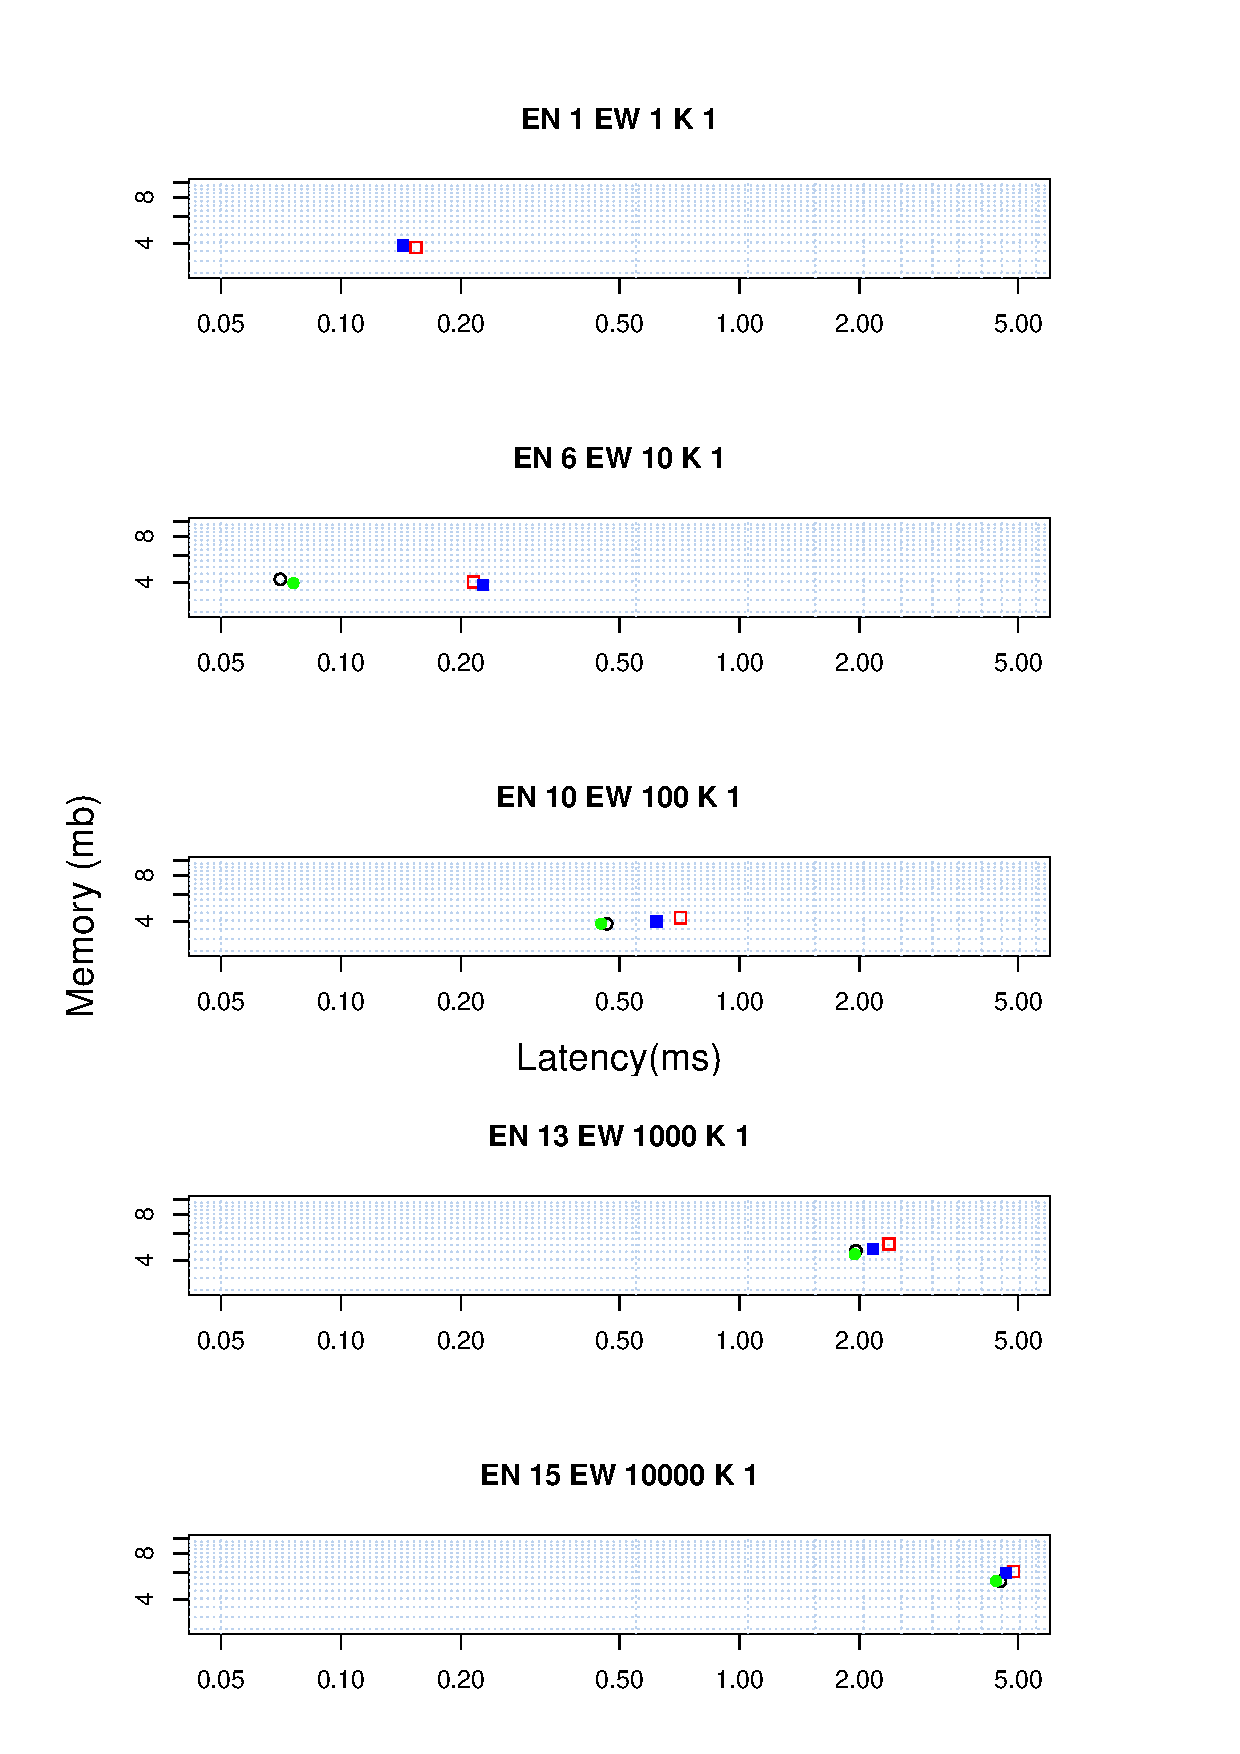
\includegraphics[width=\linewidth]{images/dashboard-1-split}	
	\caption[\textsc{Analyser} Investigation Stack - Level 0 - Dashboard One - Split Version]{Dashboard One - K=1 Split} 
	\label{fig:result_dashboard_ka}
\end{figure}
\begin{figure}[htbp]
	\centering
	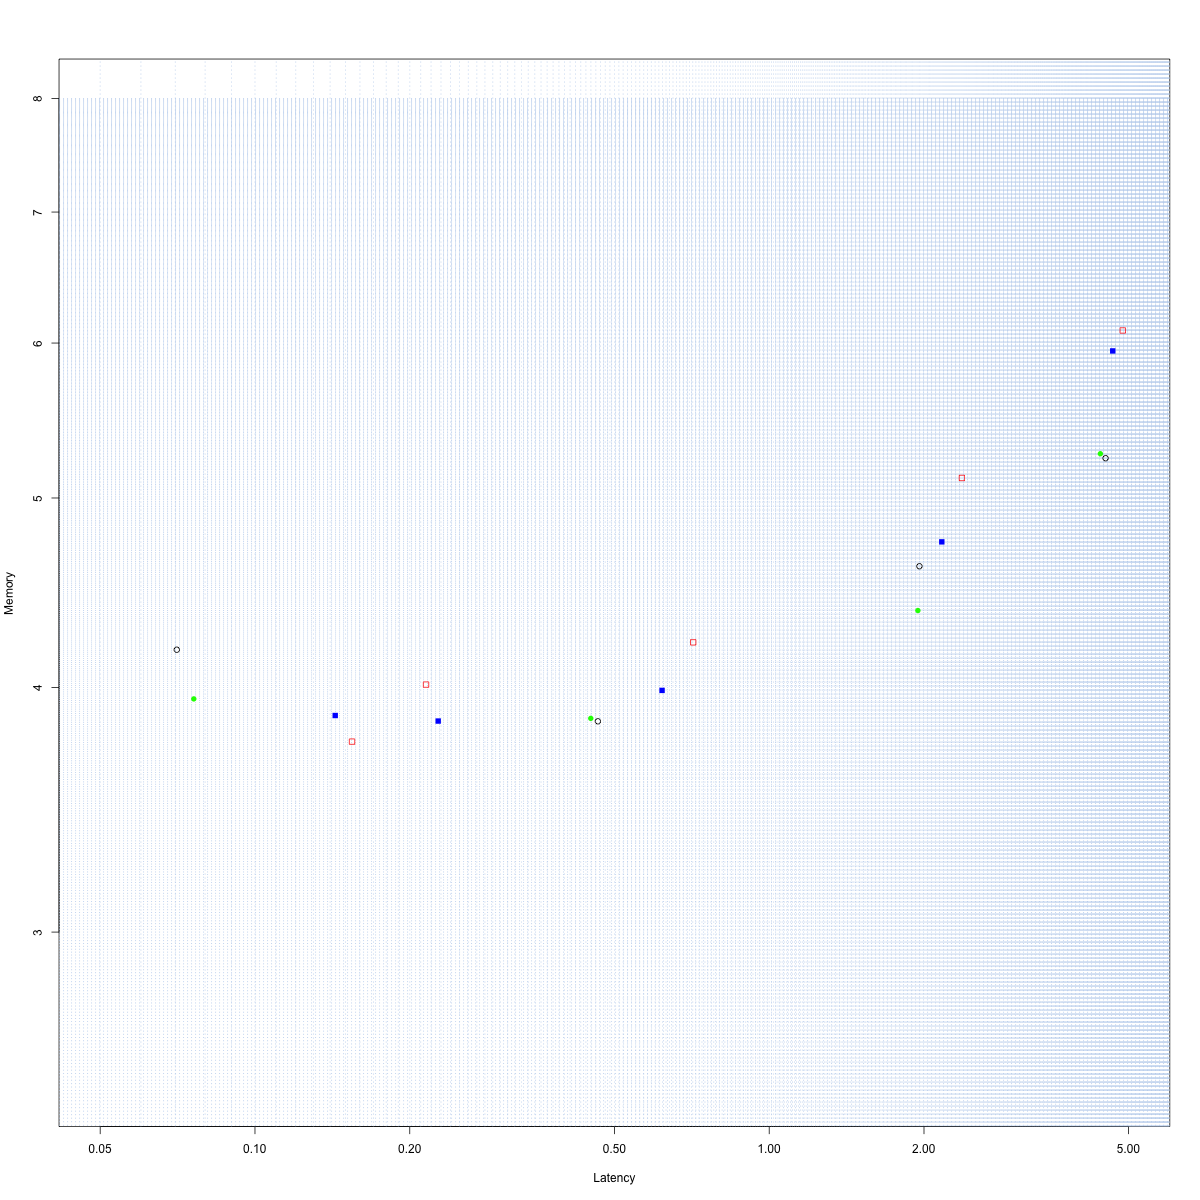
\includegraphics[width=0.90\linewidth]{images/dashboard-1}	
	\caption[\textsc{Analyser} Investigation Stack - Level 0 - Dashboard One - Multiplot Version]{Dashboard One - K=1 Multiplot} 
	\label{fig:result_dashboard_kb}
\end{figure}
\begin{figure}[htbp]
	\centering
	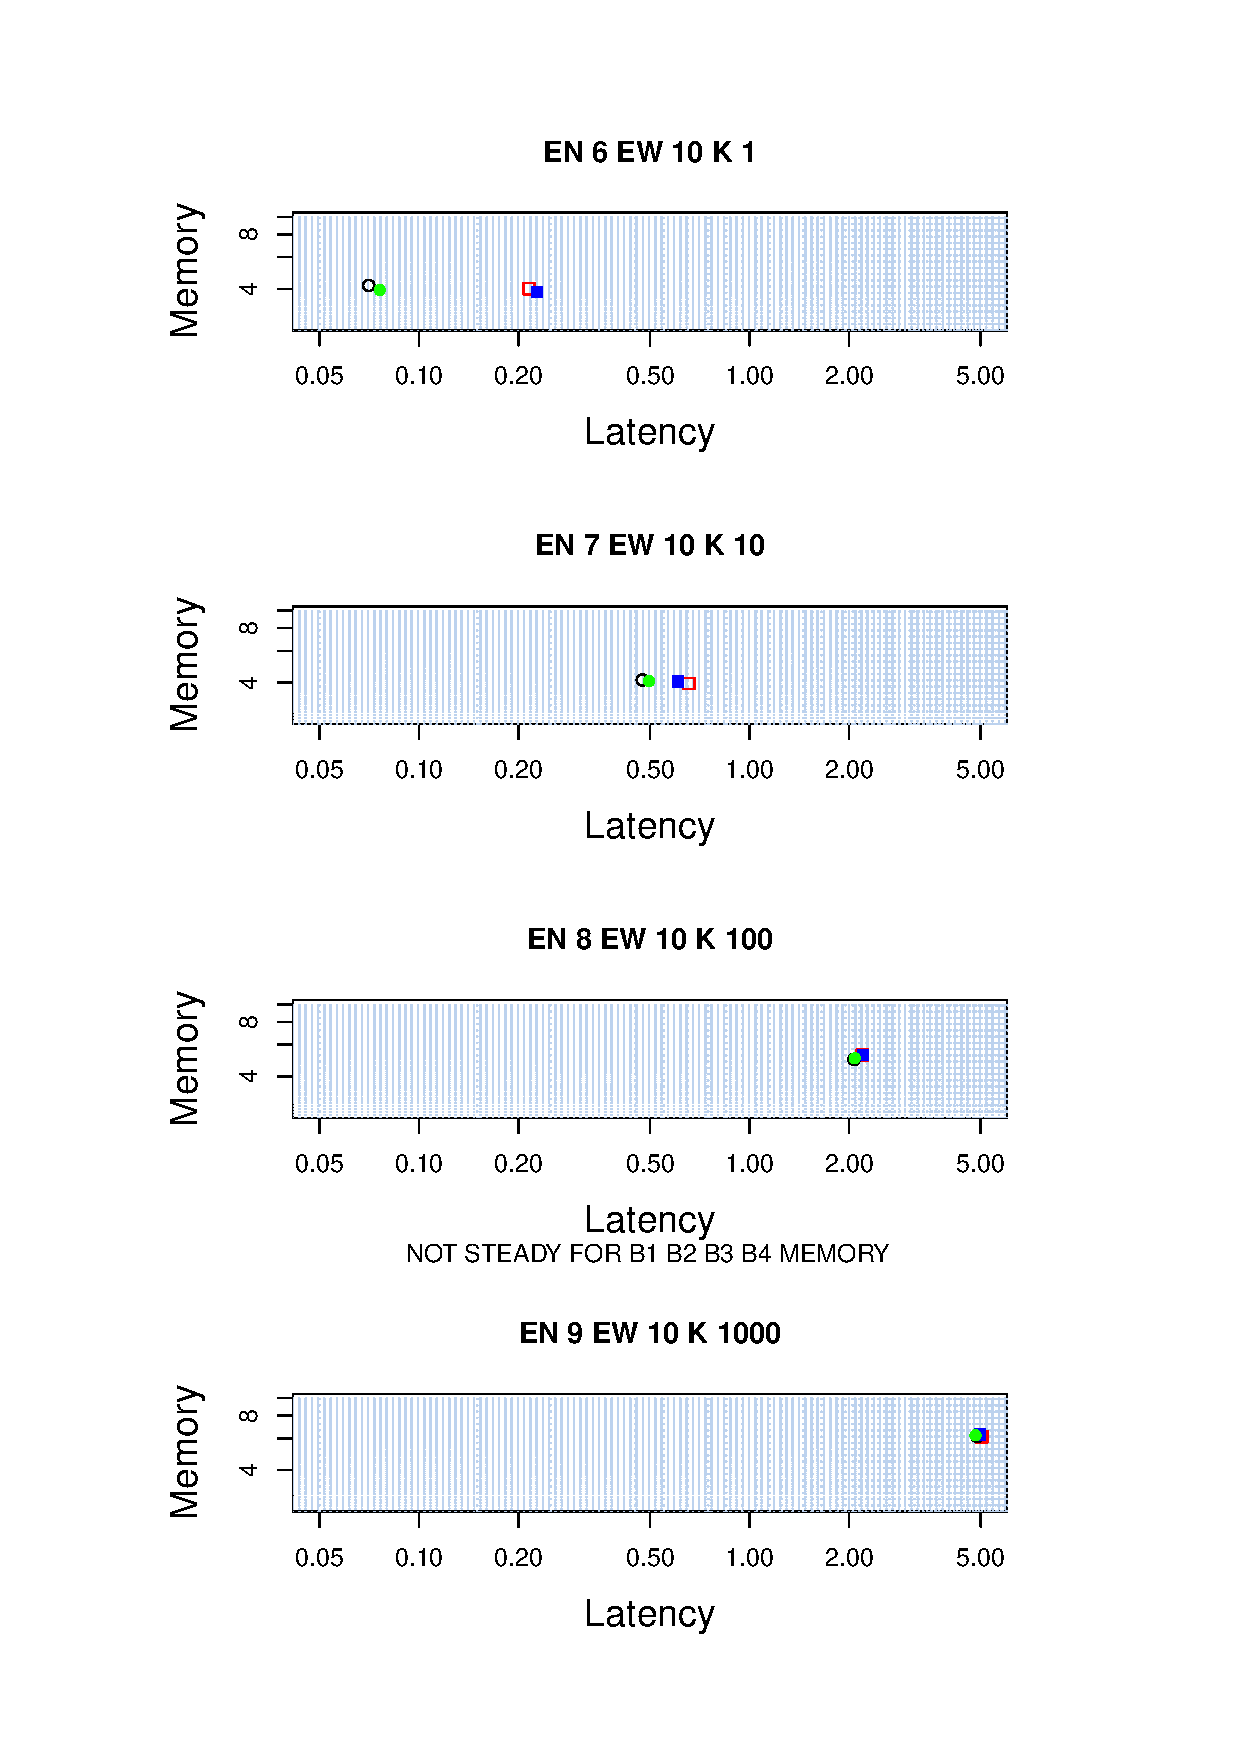
\includegraphics[width=0.90\linewidth]{images/dashboard-2-split}	
	\caption[\textsc{Analyser} Investigation Stack - Level 0 - Dashboard Two - Split Version]{Dashboard Two - EW=10 Split} 
	\label{fig:result_dashboard_ewa}
\end{figure}

\begin{figure}[htbp]
	\centering
	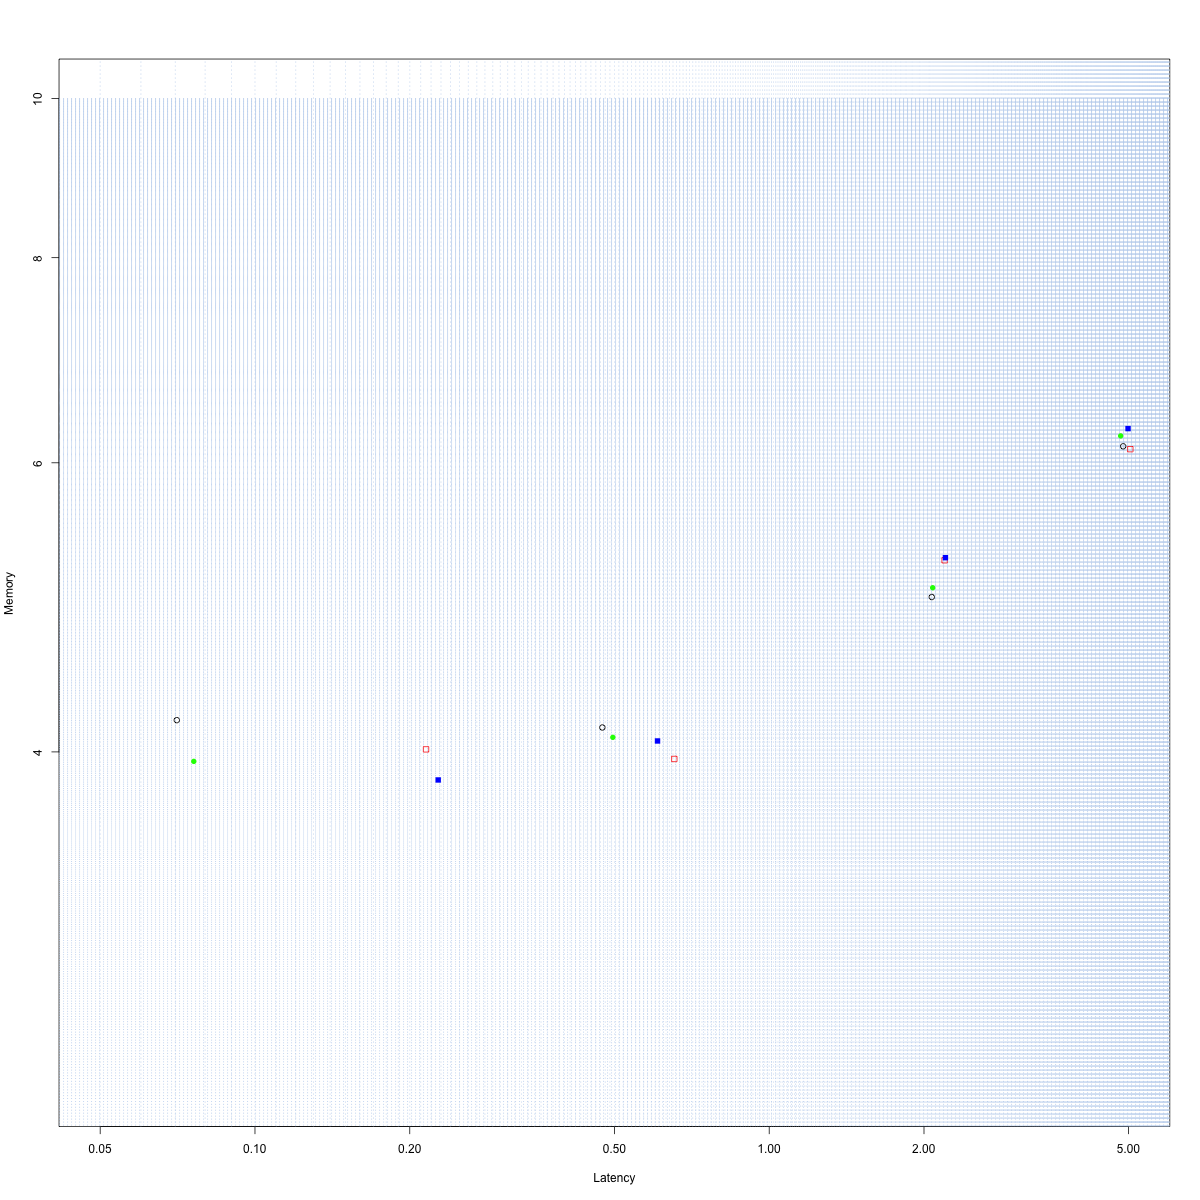
\includegraphics[width=0.90\linewidth]{images/dashboard-2}	
	\caption[\textsc{Analyser} Investigation Stack - Level 0 - Dashboard Two - Multiplot Version]{Dashboard Two - EW=10 Multiplot} 
	\label{fig:result_dashboard_ewb}
\end{figure}
\begin{figure}[htbp]
	\centering
	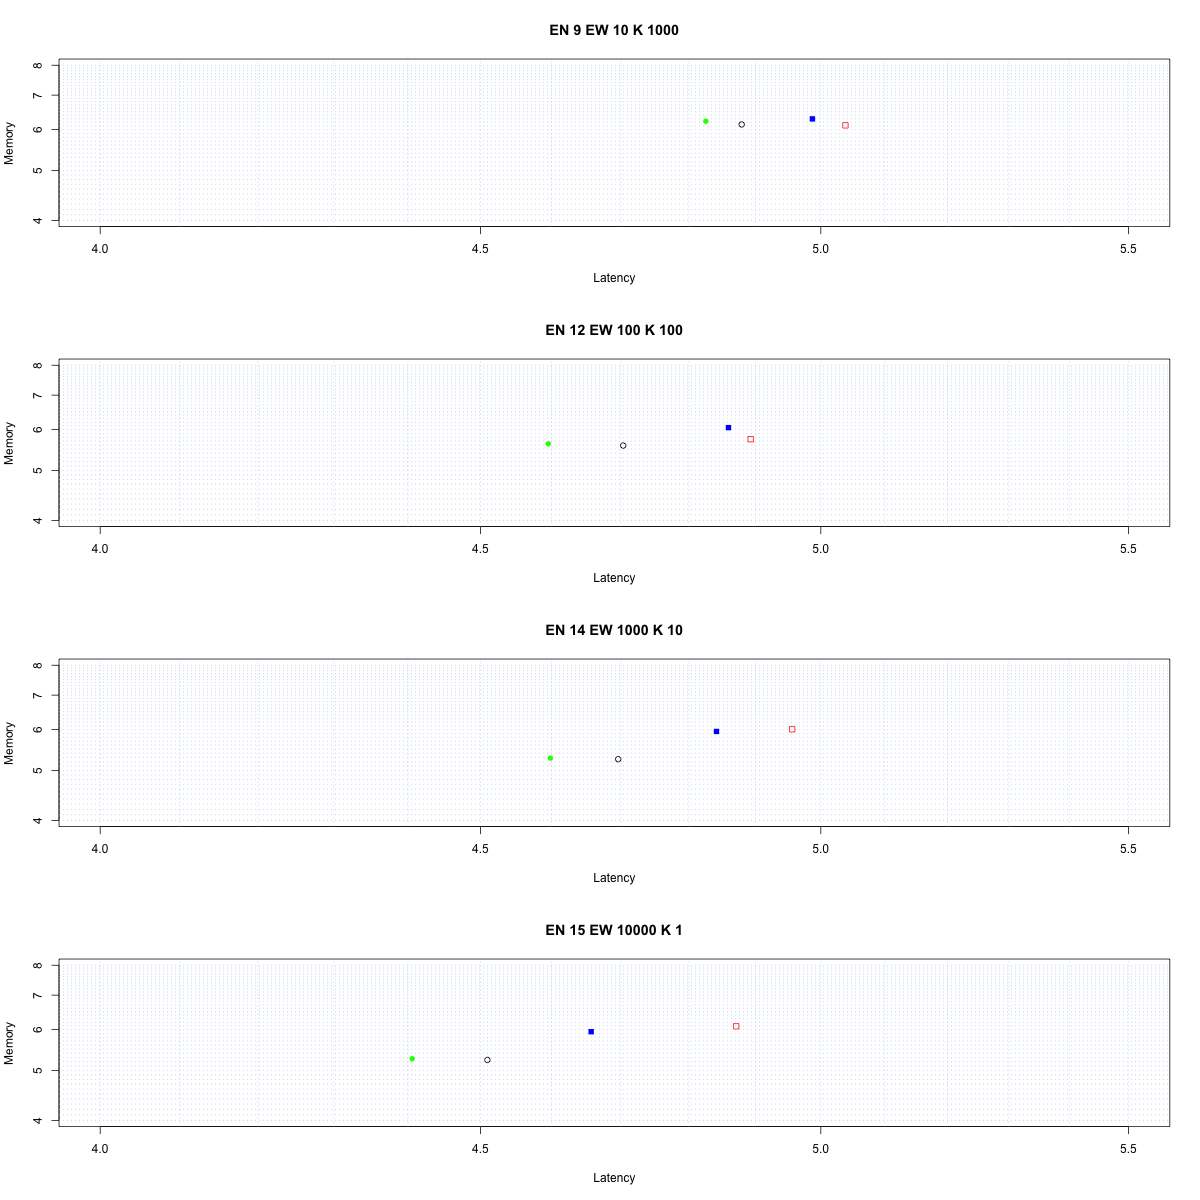
\includegraphics[width=0.90\linewidth]{images/dashboard-3-split}	
	\caption[\textsc{Analyser} Investigation Stack - Level 0 - Dashboard Three - Split Version]{Dashboard Three - $EW*K=10000$ Split} 
	\label{fig:result_dashboard_proba}
\end{figure}
\begin{figure}[htbp]
	\centering
	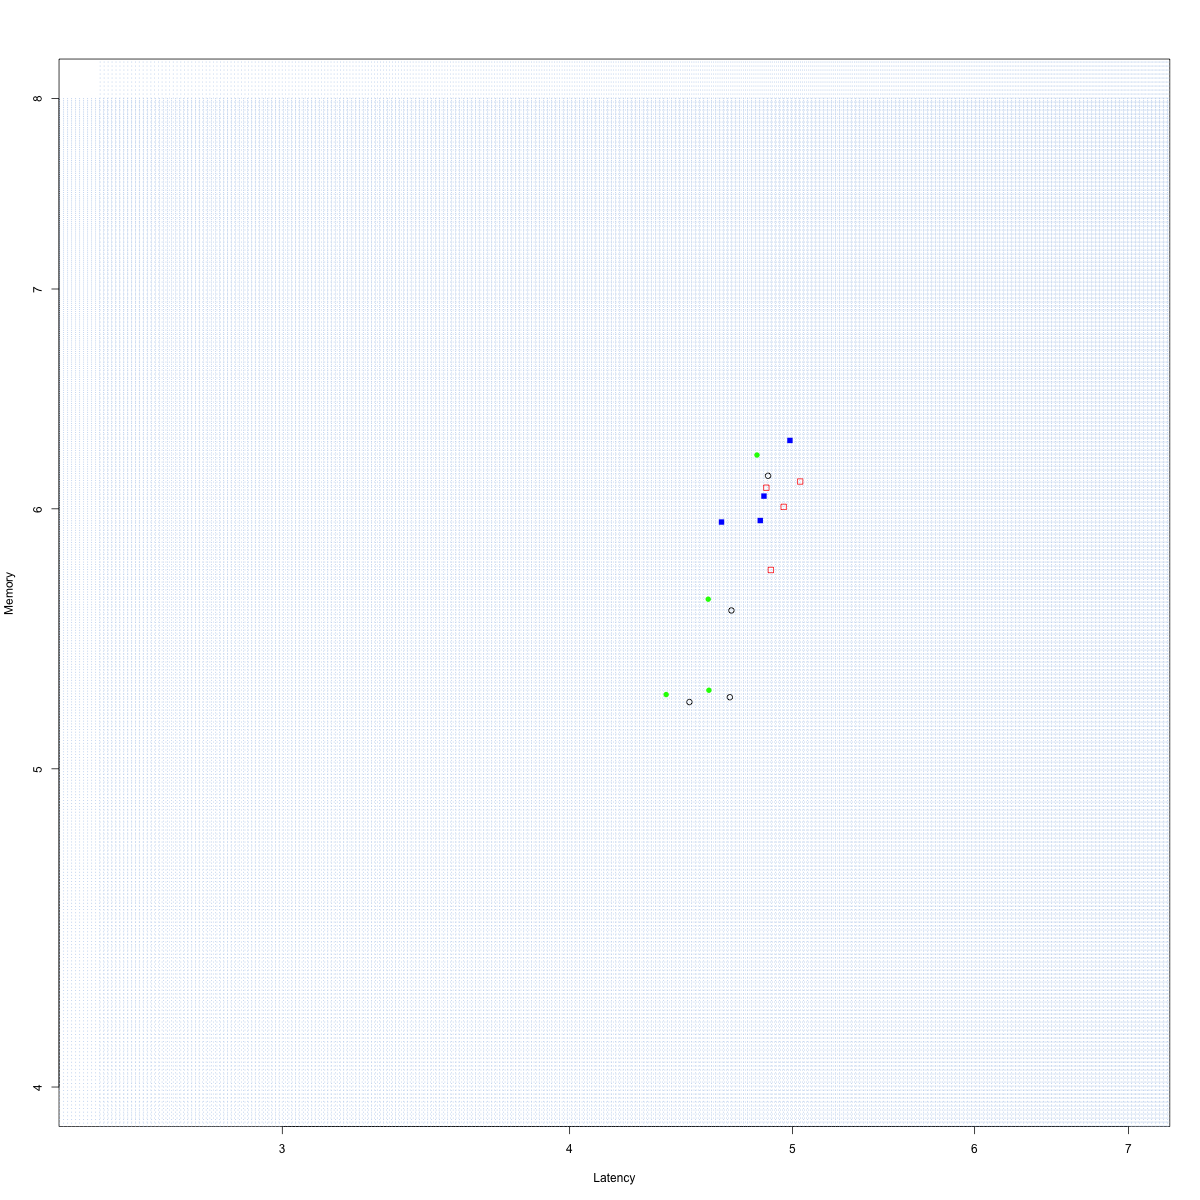
\includegraphics[width=0.90\linewidth]{images/dashboard-3}	
	\caption[\textsc{Analyser} Investigation Stack - Level 0 - Dashboard Three - Multiplot Version]{Dashboard Three - $EW*K=10000$ Multiplot} 
	\label{fig:result_dashboard_probb}
\end{figure}




\subsection{Level 1 - Statistical Values Comparison}\label{sec:eval-level1}

The Analysis Level 1 exploits statistical investigation through an easy to ready layout, which simplify the inter-experiment comparison (see~\ref{sec:analyser} Level 1).

\begin{table}[tbh]
	\centering
	\scriptsize
	\subtable[Incremental]{%
		\begin{tabular}{l | ccccc} % creating eight columns
	  	\hline
		Triple  & \multicolumn{5}{c}{Slots}  \\
		in & \multicolumn{5}{c}{Number}  \\
		Window  & 1 & 10 & 100 & 1000&10000\\
		\hline
		1	   &G	\\			
		10	   &G	&$\simeq$	\\		
		100	   &G	&$\simeq$   &	$\simeq$\\	
		1000   &	G	&$\simeq$	&$\simeq$&$\simeq$\\
		10000  &NA	&T	&S&	T	&T\\
		\hline % inserts single-line
	 \end{tabular}
	}
	\subtable[Triple]{%
		\begin{tabular}{l | ccccc} % creating eight columns
	  	\hline
		Triple  & \multicolumn{5}{c}{Slots}  \\
		in & \multicolumn{5}{c}{Number}  \\
		Window  & 1 & 10 & 100 & 1000&10000\\
		\hline
		1	&I	\\			
		10	&I	&I	\\		
		100	&N	&I&	I	\\	
		1000&	N&	I	&I	&I\\	
		10000&	NA	&I	&I	&I	&I\\
		\hline % inserts single-line
		\end{tabular}
	}	
	\subtable[Naive]{%
		\begin{tabular}{l | ccccc} % creating eight columns
	  	\hline
		Triple  & \multicolumn{5}{c}{Slots}  \\
		in & \multicolumn{5}{c}{Number}  \\
		Window  & 1 & 10 & 100 & 1000 &10000\\
		\hline
		1	 &$\simeq$\\				
		10	 &$\simeq$&$\simeq$	\\		
		100	 &G	      &$\simeq$&	T\\		
		1000	 &G	      &$\simeq$	&T	&T	\\
		10000&NA	      &$\simeq$	& 	$\simeq$	&T	&T\\
		\hline % inserts single-line
	 	\end{tabular}
	}
	\subtable[Graph]{%
		\begin{tabular}{l | ccccc} % creating eight columns
	  	\hline
		Triple  & \multicolumn{5}{c}{Slots}  \\
		in & \multicolumn{5}{c}{Number}  \\
		Window  & 1 & 10 & 100 & 1000 &1000\\
		\hline			
		1	&I	\\			
		10	&I	&I		\\	
		100	& $\simeq$	&I	&I		\\
		1000 &	N	&I	&I	&I	\\
		10000&	NA	&I	&I	&I	&I\\
		\hline % inserts single-line
		\end{tabular}
	}
	\caption[\textsc{Analyser} Investigation Stack - Level 1 - SOAK Test Average Latency Comparison]{\textsc{Analyser} Investigation Stack - Level 1 - SOAK Test average latency comparison trough a qualitative approach. The following convention indicates the baseline has not reached the Steady State Condition:
	\underline{G}, \underline{T}, \underline{N}, \underline{I}.
	(a), (c) - latency results comparison between Incremental and Naive approaches; (b), (d) - latency results comparison between Graph-based and Triple-based models.}
	\label{tab:soak_latency_comparisons}	
\end{table}

The current evaluation operates over the average values of latency and memory. Tables~\ref{tab:soak_latency_comparisons} and~\ref{tab:soak_memory_comparisons} contain in all the experiment results respectively for latency and memory.  Both the tables dispose the results according with the layout of Table~\ref{tab:soaktests-alt}. We decide to use the qualitative result representation, but \name allows also more detailed analysis with quantitative comparisons as shows in Section~\ref{sec:analyser-impl}. To properly read the tables note that they report that baseline is better than another one when the difference in term of latency or memory is bigger than 5\%, otherwise we consider the two terms of comparison as equal and we use the simble $\simeq$.
Moreover, we indicate that the better solution has not reached the Steady State Condition with the underlined symbols \underline{G}, \underline{T}, \underline{N}, \underline{I}.


\begin{table}[tbh]
	\centering
	\scriptsize
	\subtable[Incremental]{%
		\begin{tabular}{l | ccccc} % creating eight columns
	  	\hline
		Triple  & \multicolumn{5}{c}{Slots}  \\
		in & \multicolumn{5}{c}{Number}  \\
			Window  & 1 & 10 & 100& 1000&10000\\
		\hline
		1  	  & T\\
		10    & G     &  	T  \\
		100   & G     & 	T  & G\\
		1000  & \underline{G}     & 	\underline{G}  & \underline{G} & \underline{T} \\
		10000 &NA     & G  & G & G&G\\
		\hline % inserts single-line
	 \end{tabular}
	}
	\subtable[Triple]{%
		\begin{tabular}{l | ccccc} % creating eight columns
	  	\hline
		Triple  & \multicolumn{5}{c}{Slots}  \\
		in & \multicolumn{5}{c}{Number}  \\
			Window  & 1 & 10 & 100& 1000&10000\\
		\hline
		1    & N\\
		10   & I   & N \\
		100   & N & N & I\\
		1000 & \underline{N} & \underline{I} & \underline{I} & \underline{I}\\
		10000 & NA & I & I & I & I\\
		\hline % inserts single-line
		\end{tabular}
	}	

	\subtable[Naive]{%
		\begin{tabular}{l | ccccc} % creating eight columns
	  	\hline
		Triple  & \multicolumn{5}{c}{Slots}  \\
		in & \multicolumn{5}{c}{Number}  \\
			Window  & 1 & 10 & 100& 1000&10000\\
		\hline
		1  	  & G\\
		10    & G  &  	T \\
		100   & G  & 	G  & T\\
		1000  & \underline{G}  & 	\underline{G}  & \underline{G} & \underline{T}\\
		10000 & NA & 	G  & G & T &T\\
		\hline % inserts single-line
	 	\end{tabular}
	}
	\subtable[Graph]{%
		\begin{tabular}{l | ccccc} % creating eight columns
	  	\hline
		Triple  & \multicolumn{5}{c}{Slots}  \\
		in & \multicolumn{5}{c}{Number}  \\
		Window  & 1 & 10 & 100& 1000&10000\\
		\hline
		1       & N\\
		10      & N        & N \\
		100     & $\simeq$ & N & I \\
		1000    & \underline{$\simeq$} & \underline{I} & \underline{I} & \underline{I} \\
		100000  & NA       & N & I & I & I \\
		\hline % inserts single-line
		\end{tabular}
	}	
	\caption[\textsc{Analyser} Investigation Stack - Level 1 - SOAK Test Average Memory Comparison]{The following convention indicates the baseline has not reached the Steady State Condition:
	\underline{G}, \underline{T}, \underline{N}, \underline{I}. 
	(a), (c) - memory results comparison between Incremental and Naive approaches; (b), (d) - memory results comparison between Graph-based and Triple-based models}
	\label{tab:soak_memory_comparisons}	
\end{table}

When $N>$1, the results in Table~\ref{tab:soak_latency_comparisons}.a and~\ref{tab:soak_latency_comparisons}.c allow to say that using a Triple-base RDF stream is faster than Graph-based one. In particular, for the case $N$=1000 when the window contains 1000 triples (i.e., each \textsc{CTEvent} contains only one triple),  the Naive Triple-based approach is about 10\% faster  than the Naive Graph-based one while the Incremental Graph-based is even about 20\% faster. This findings confirm [Hp.2], while the cases  when N=10 the does not confirm the hypothesis because the results can be consider as equal (result differences are smaller than 5\%). A possible explanation is that the dimension of the graph can not be considered small w.r.t the window when $N$=10.

When $N$=1 (i.e., the window contains only one \textit{CTEvent}) instead, the results in Table~\ref{tab:soak_latency_comparisons}.b and Table~\ref{tab:soak_latency_comparisons}.d show that for large events the Naive approach is faster than the Incremental one, as we stated when we formulate [Hp.1]. Instead, when \textit{CTEvent} contains only few triples, the Incremental approach is faster and this is not intuitive, because to formulate [Hp.1] we consider the changes dimension in percentage.

The results in Table~\ref{tab:soak_latency_comparisons}.b and~\ref{tab:soak_latency_comparisons}.d support [Hp.1] by stating that when the number of changing triples in $\Delta+ \Delta-$ (Section~\ref{sec:baselines}) is a small fraction of those in the window an Incremental approach is faster than the Naive one. The exception of case $N$=1, but it can be seen as a limit case, where the reasoner is asked to deduce all the implicit triples implied by the only explicit triple in the window.  

While is possible to state meaningful observation over latency data, the same is not possible for memory ones. \name shows that the study of the memory can not be faced with the same methods to study latency (comparison of the average values under a clearly identified the Steady State condition). 

Table~\ref{tab:soak_memory_comparisons} reports the results for the memory usage during the experiments. Table entries do not confirm what we observed in Table~\ref{tab:soak_latency_comparisons} and sometimes it even refutes our findings. It is clear that memory usage does not follow the same behaviour of latency, even if [Hp.1] and [Hp.2] are not totally refused by the results.

Further statistical analysis are certainly meaningful. Comparing maximum or minimum as we did for the average values may detail much more the system memory usage. %through \name it is possible explore completely the analysis at a certain level, or we can lead the analysis to another level, following the inspected results we obtained.

\subsection{Level 2 - Patter Identification}\label{sec:eval-level2}

Statistical analysis are meaningful, but may reduce too much the RSP Engine complexity by focusing on single element of comparison. A more complete analysis is required and \name can investigate the behaviour of the system over all the experiment execution.

Level 2 exploits again the layout of Table~\ref{tab:soaktests-alt}, disposing in table cell a graphical representation of a certain variable (Latency, Memory). The graphical representation choice depends on the research necessities: time domain representations and value distribution are the ones we explored during our evaluation, both in log scale or linear scale.

\begin{figure}[h!tbp]
  \centering
	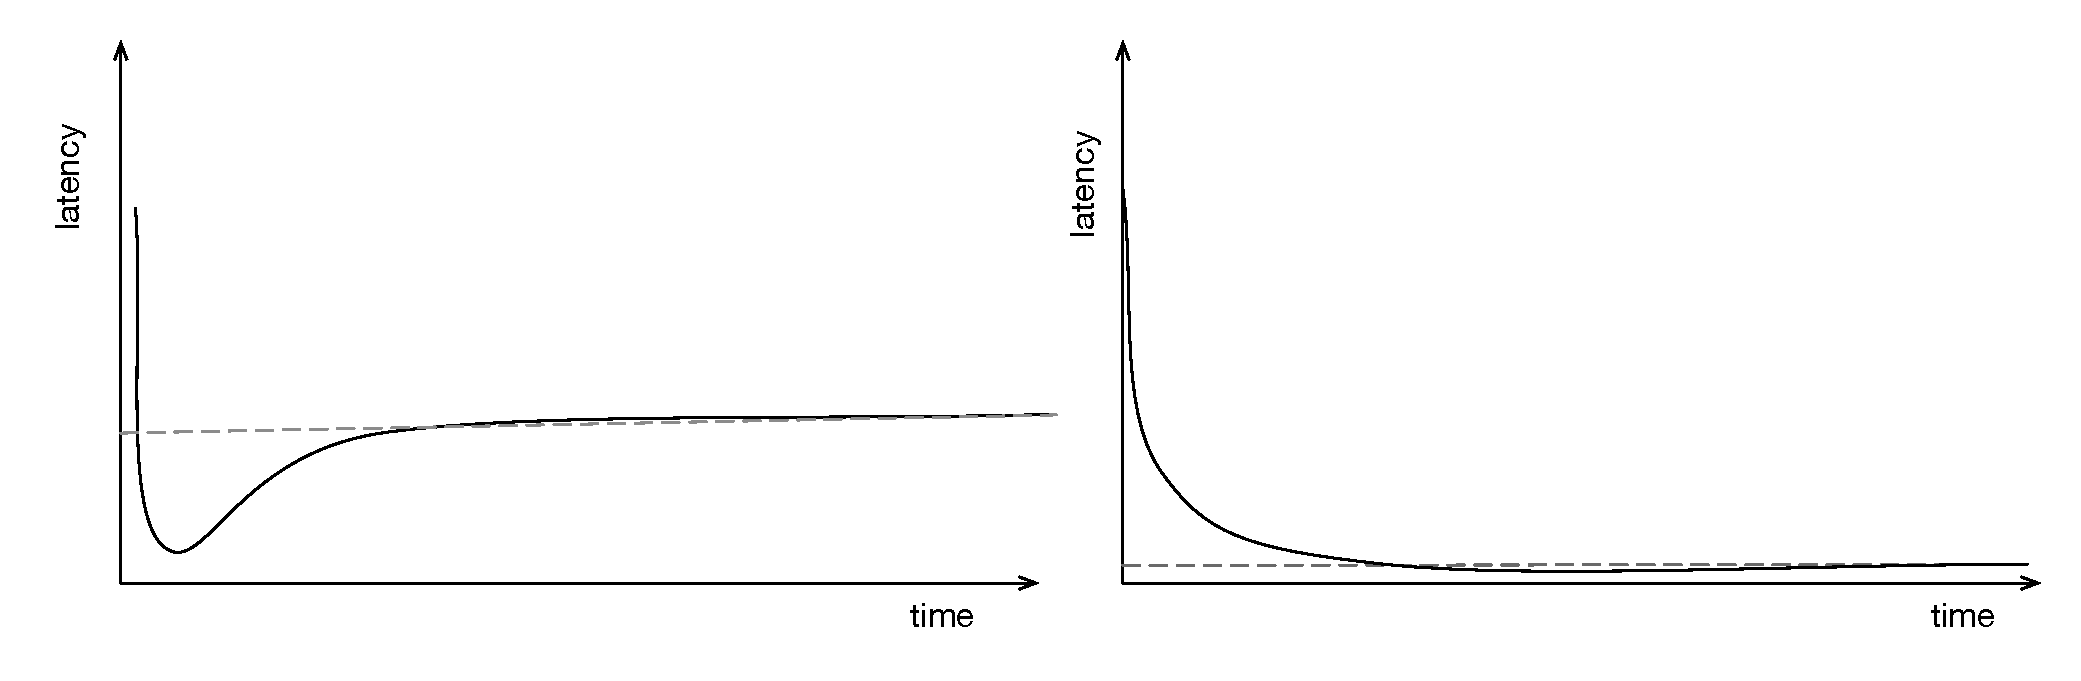
\includegraphics[width=\linewidth]{images/level2-pattern}
	\caption[\textsc{Analyser} Investigation Stack - Level 2 - Recognised Latency Patterns for SOAK Experiments]{Recognised Latency Pattern for SOAK Experiments} 
  	\label{fig:level2-pattern}
\end{figure}

The Tables~\ref{tab:level2-latency-graph} and~\ref{tab:level2-latency-triple} represent in linear scale the latency time series of the four Baselines. Immediately we can see that most of the systems reach a Steady State condition in a short period, between the 10\% and the 20\% of the entire experiment duration. Some of them show filling phenomena, when the sizes of the window start to be relevant w.r.t. the experiment duration. In general, the latency trend follows one of the pattern showed in Table~\ref{fig:level2-pattern}. %Moreover, the responsiveness is not guaranteed for the biggest experiments, especially during the warm-up phase.

The Tables~\ref{tab:level2-memory-graph} and~\ref{tab:level2-memory-triple} show the representation in linear scale of the memory time series of the four Baselines. Despite what happens for latency, we can observe that the memory usage does not reach a Steady State condition for all the experiments (Baseline GI and TI for windows of dimension 1000 Triples with more than one slot).  To reach the Steady State condition for memory, the system requires from 3.000 to 25.000 \textsc{CTEvent}s, but in general it has not a common behaviour. The variance of these results is high and can be motivated arguing about how Java is managing the memory during the execution. The optimisation policies work better when the system have to handle a lot of triples. The proof of this insight can be seen in Tables~\ref{tab:level2-memory-graph} and~\ref{tab:level2-memory-triple}. The lower levels of the Tables reach the Steady State condition before the higher ones. For those experiments that involved GI and TI, the Baselines with an incremental reasoning approach, the Steady State is not even reached, maybe because the memory consume does not alert the JVM at all. 

The filling phenomena we identified for latency are still visible in both the tables. This denotes the existence of a relation between memory and latency. This is one of the point we can further investigate through the next analysis step: Level 3.

Tables~\ref{tab:level2-memory-density-graph} and~\ref{tab:level2-memory-density-triple} represent the distribution of memory time series values of the four Baselines. To obtain this representation we individuate the minimum and the maximum between all the experiments. We divided the span in some intervals and automatically we count how many values of the memory time series fit the intervals, repeating this count for all the experiment. through this representation we can see how the memory usage is distributed during the experiment execution. We can observe that the memory values for the baselines that exploit incremental reasoning, GI and TI, are distributed in a smaller interval w.r.t the baselines which exploit the Naive reasoning approach and thus GI and T I have a smarter usage of the memory. When the window size increases, the memory consumption shift to the right, towards the intervals with higher values.

All the four tables about memory time series and memory distribution show that there are strong difference between the experiment subset with window dimension of 1000  triples and the ones with window dimension 10000 triples. This is a meta-insight that improves the Experiment Design model. Actually we are still not able to predict the baselines behaviour, but we can further investigate through \namens.

The quantitative nature of the hypothesis formulated in Section~\ref{sec:soak-es} does not allow to exploit Level 2 for Hypothesis verification. Actually [Hp.1] and [Hp.2] consider the performance as the main evaluation metric, while Level 2 fulfils the necessity to understand the system nature. The insights above allow to improve the RSP Engine model, upon which is possible to formulate more precise hypothesis and to explain the unpredictable results we obtained from Level 0 and Level 1.

\subsection{Level 3 - Single Visual Comparison}\label{sec:eval-level3}
	
Level 3 operates a drill down from Level 2, providing examples of \textit{Intra Experiment} comparisons, in order to highlight the relation between memory and latency performances. Level 2 has shown several differences that can explain the absence of a dominant Baseline solution over all the experiment and w.r.t [Hp.1] and [Hp.2]. Thus Level 3 starts from three important findings:
\begin{itemize}
\item All the experiments reach the Steady State for latency, but several of them do not reach it for memory.
\item When the Steady State condition is reached: latency requires about 2.000-5.000 \textsc{CTEvent}s w.r.t the total experiment duration of 30.000, while memory requires from 5.000 to 25.000 \textsc{CTEvent}s.
\item Both memory and latency analysis show the presence of filling phenomena, which should be further investigated.
\end{itemize}

Figure~\ref{fig:level3-not-steady-naive-graph-en11} contains two examples of experiment that reach the Steady State condition for latency but not for memory. Figure~\ref{fig:level3-not-steady-naive-graph-en11}.a shows the latency and memory usage for the Baseline GN within the experiment eleven (\textsc{CTEvent} size = 10, Number of Slot = 100), Figure~\ref{fig:level3-not-steady-naive-graph-en11}.b shows the latency and memory usage of the Baseline TI, within the same experiment. 

If we consider only the memory trend, we note an oscillating behaviour which contrast with the idea of Steady State. A more careful analysis identifies the presence of some spikes in the latency time series. It represents a certain period of time where the content of the window requires a strong reasoning effort. This may also influence the memory usage. Moreover, this kind of analysis can not be seen from higher level. 

Figure~\ref{fig:level3-steady-naive-graph-en12-7} (a) and (b) show two examples of steady state condition reaching. The figure~\ref{fig:level3-steady-naive-graph-en12-7}.a describes that the Baseline GN for experiment seven (\textsc{CTEvent} size = 10, Number of Slot = 10) reaches the Steady State around the 10\% of the entire experiment duration for latency and about 45\% for memory. 
Java probably focuses on speeding up the execution rather than saving resources. A completely different behaviour can be appreciate in the subfigure (b), where both latency and memory reach the Steady State around the 10\% of the entire execution. It seems that bigger is the amount of resources required by the program, faster Java's optimization policies work.

Figures~\ref{fig:level3-filling-inc-stmt-en15} (a) and (b) show the relation between the filling phenomena together for latency and memory for the Baselines TN and TI within Experiment 15 ( \textsc{CTEvent} size = 1 Num. Slots = 10000). The main insight regards how Java manages the initial warm-up phase. We have seen that the JVM usually over-estimates the necessary amount of memory at the beginning of the execution, then it tries to optimize. When the window dimension in terms of triple is increasing the memory occupation has a worsening and latency follows the same behaviour. Finally, latency and memory reach the stability when the filling phenomenon ends, since the number of triples in the active window is now constant.

\begin{table}[htbp]
	\centering
	\scriptsize
	\subtable[Graph Naive]{%
		\begin{tabular}{l | ccccc} % creating eight columns
	  	\hline
		Triple  & \multicolumn{5}{c}{Slots}  \\
		in & \multicolumn{5}{c}{Number}  \\
		Window  & 1 & 10 & 100 & 1000&10000\\
		\hline
		\hline
		1	   &\begin{minipage}{.15\textwidth}
				\vspace{2pt}
     			 	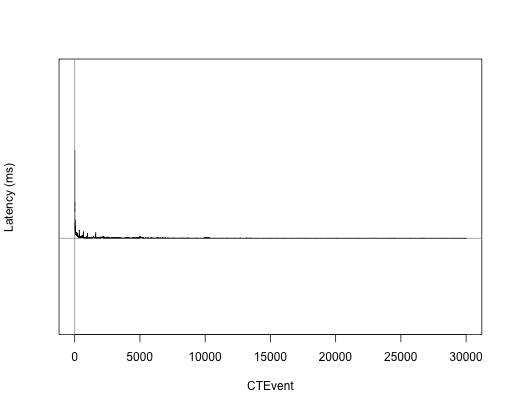
\includegraphics[width=\linewidth]{images/lat-log-graph/N1}
    				 \end{minipage}\\			
		10	   & \begin{minipage}{.15\textwidth}
     			 	
				\vspace{2pt}
     			 	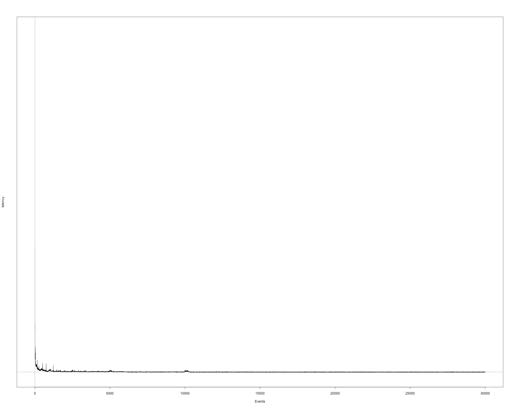
\includegraphics[width=\linewidth]{images/lat-log-graph/N2}
    				\end{minipage}
    			   & \begin{minipage}{.15\textwidth}
     			 	
				\vspace{2pt}
     			 	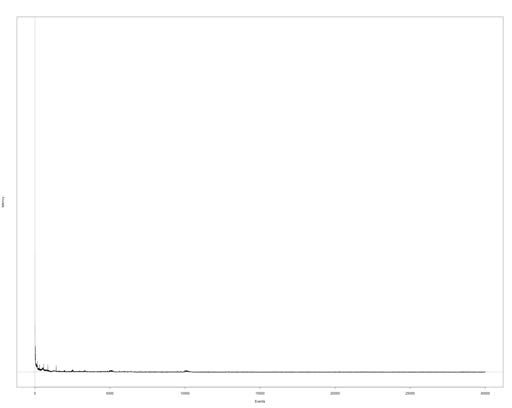
\includegraphics[width=\linewidth]{images/lat-log-graph/N6}
    				 \end{minipage}\\		
		100	   & \begin{minipage}{.15\textwidth}
     			 	
				\vspace{2pt}
     			 	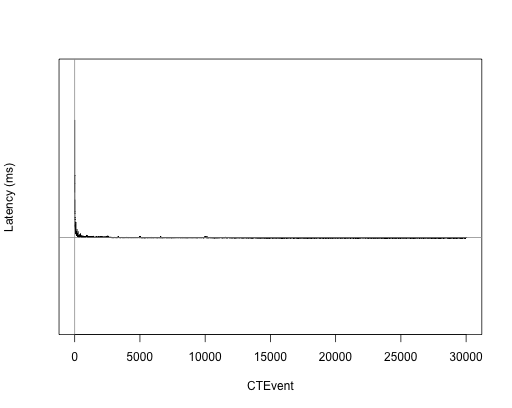
\includegraphics[width=\linewidth]{images/lat-log-graph/N3}
    				 \end{minipage}
    			   & \begin{minipage}{.15\textwidth}
     			 	
				\vspace{2pt}
     			 	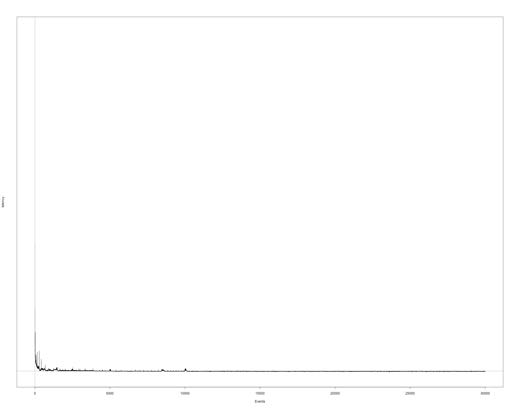
\includegraphics[width=\linewidth]{images/lat-log-graph/N7}
    				 \end{minipage}
    			   &	 \begin{minipage}{.15\textwidth}
     			 	
				\vspace{2pt}
     			 	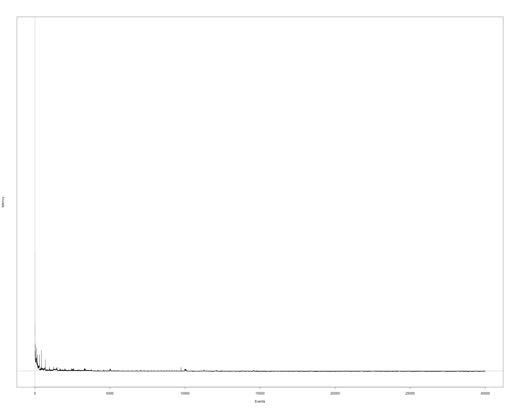
\includegraphics[width=\linewidth]{images/lat-log-graph/N10}
    				 \end{minipage}\\	
		1000   &	 \begin{minipage}{.15\textwidth}
     			 	
				\vspace{2pt}
     			 	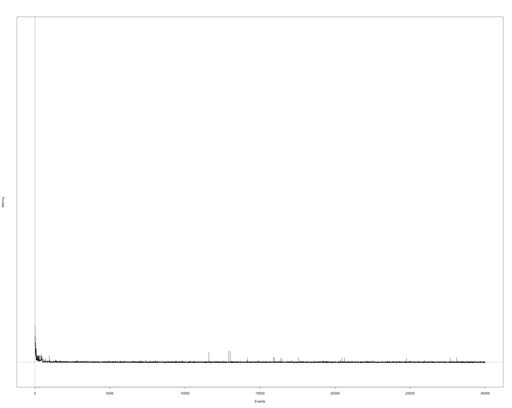
\includegraphics[width=\linewidth]{images/lat-log-graph/N4}
    				 \end{minipage}
    			   &	 \begin{minipage}{.15\textwidth}
     			 	
				\vspace{2pt}
     			 	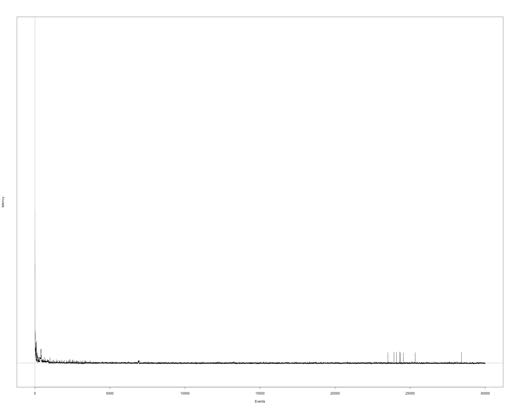
\includegraphics[width=\linewidth]{images/lat-log-graph/N8}
    				 \end{minipage}
    			   &	 \begin{minipage}{.15\textwidth}
     			 	
				\vspace{2pt}
     			 	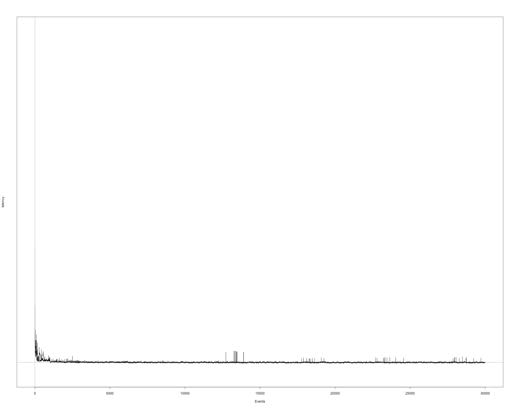
\includegraphics[width=\linewidth]{images/lat-log-graph/N11}
    				 \end{minipage}
    			   &	 \begin{minipage}{.15\textwidth}
     			 	
				\vspace{2pt}
     			 	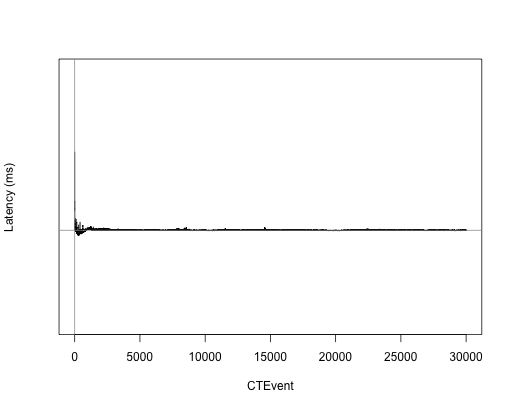
\includegraphics[width=\linewidth]{images/lat-log-graph/N13}
    				 \end{minipage}\\
		10000  &	 \begin{minipage}{.15\textwidth}
     			 	
				\vspace{2pt}
     			 	
\includegraphics[width=\linewidth]{images/lat-log-graph/N5}
    				 \end{minipage}
    			   &	 \begin{minipage}{.15\textwidth}
     			 	
				\vspace{2pt}
     			 	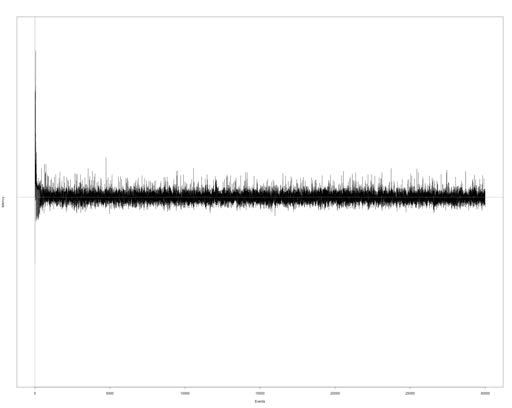
\includegraphics[width=\linewidth]{images/lat-log-graph/N9}
    				 \end{minipage}
    			   &	 \begin{minipage}{.15\textwidth}
     			 	
				\vspace{2pt}
     			 	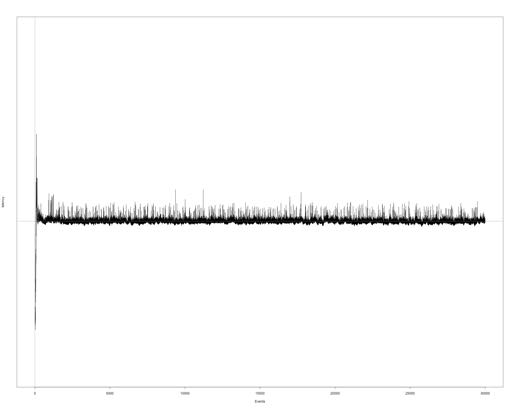
\includegraphics[width=\linewidth]{images/lat-log-graph/N12}
    				 \end{minipage}
    			   &	 \begin{minipage}{.15\textwidth}
     			 	
				\vspace{2pt}
     			 	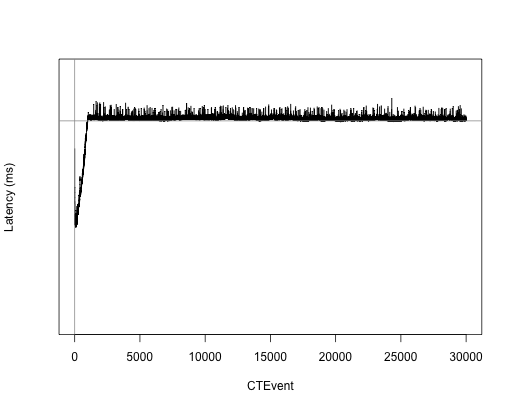
\includegraphics[width=\linewidth]{images/lat-log-graph/N14}
    				 \end{minipage}
    			   &	 \begin{minipage}{.15\textwidth}
     			 	
				\vspace{2pt}
     			 	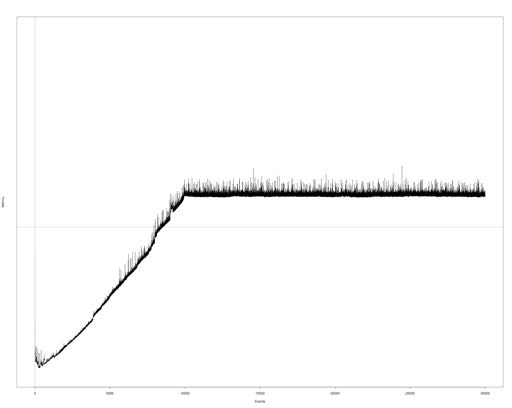
\includegraphics[width=\linewidth]{images/lat-log-graph/N15}
    				 \end{minipage}\\
		\hline % inserts single-line
	 \end{tabular}
	}
	\subtable[Graph Incremental]{%
		\begin{tabular}{l | ccccc} % creating eight columns
	  	\hline
		Triple  & \multicolumn{5}{c}{Slots}  \\
		in & \multicolumn{5}{c}{Number}  \\
		Window  & 1 & 10 & 100 & 1000&10000\\
		\hline
			\hline
		1	   &\begin{minipage}{.15\textwidth}
     			 	
				\vspace{2pt}
     			 	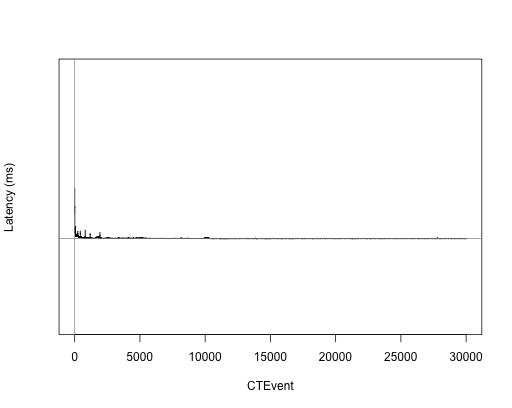
\includegraphics[width=\linewidth]{images/lat-log-graph/I1}
    				 \end{minipage}\\			
		10	   & \begin{minipage}{.15\textwidth}
     			 	
				\vspace{2pt}
     			 	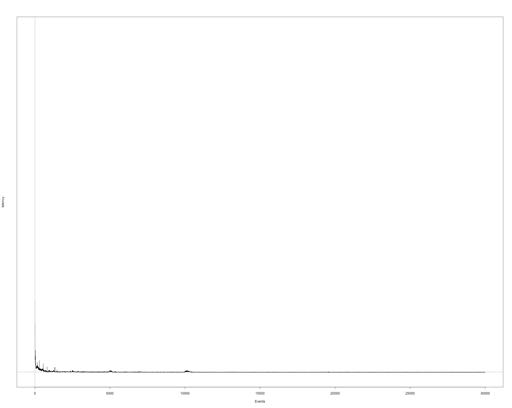
\includegraphics[width=\linewidth]{images/lat-log-graph/I2}
    				\end{minipage}
    			   & \begin{minipage}{.15\textwidth}
     			 	
				\vspace{2pt}
     			 	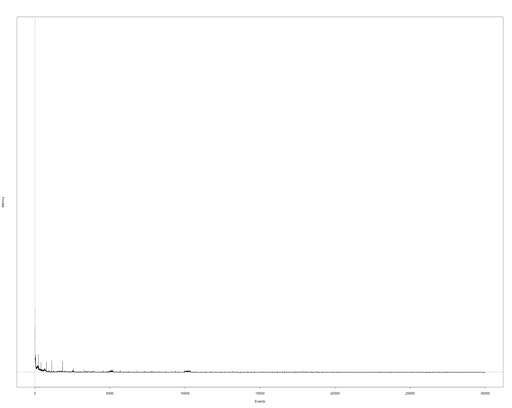
\includegraphics[width=\linewidth]{images/lat-log-graph/I6}
    				 \end{minipage}\\		
		100	   & \begin{minipage}{.15\textwidth}
     			 	
				\vspace{2pt}
     			 	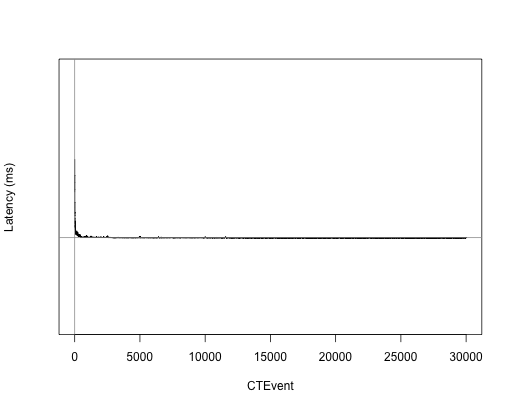
\includegraphics[width=\linewidth]{images/lat-log-graph/I3}
    				 \end{minipage}
    			   & \begin{minipage}{.15\textwidth}
     			 	
				\vspace{2pt}
     			 	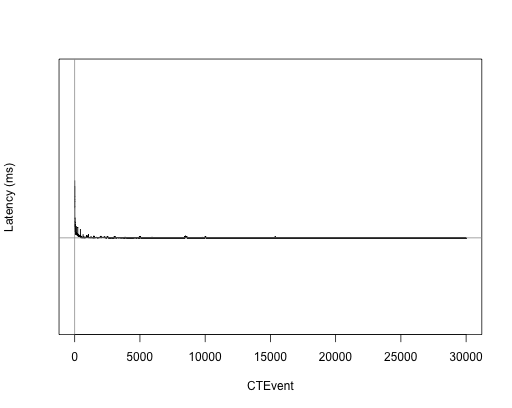
\includegraphics[width=\linewidth]{images/lat-log-graph/I7}
    				 \end{minipage}
    			   &	 \begin{minipage}{.15\textwidth}
     			 	
				\vspace{2pt}
     			 	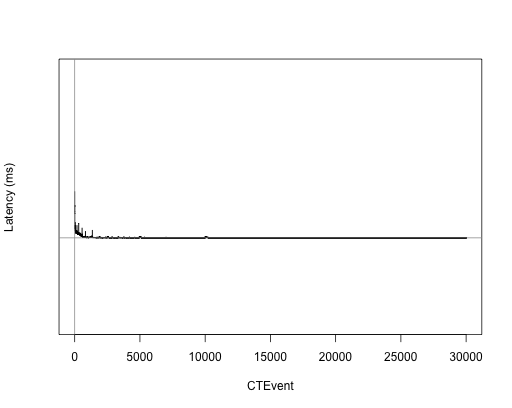
\includegraphics[width=\linewidth]{images/lat-log-graph/I10}
    				 \end{minipage}\\	
		1000   &	 \begin{minipage}{.15\textwidth}
     			 	
				\vspace{2pt}
     			 	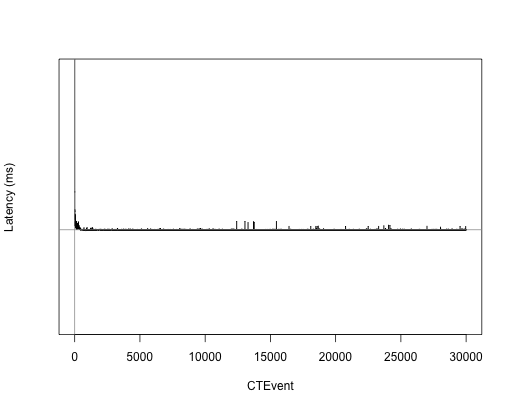
\includegraphics[width=\linewidth]{images/lat-log-graph/I4}
    				 \end{minipage}
    			   &	 \begin{minipage}{.15\textwidth}
     			 	
				\vspace{2pt}
     			 	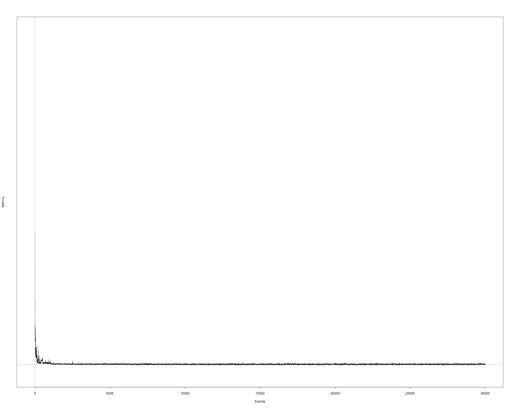
\includegraphics[width=\linewidth]{images/lat-log-graph/I8}
    				 \end{minipage}
    			   &	 \begin{minipage}{.15\textwidth}
     			 	
				\vspace{2pt}
     			 	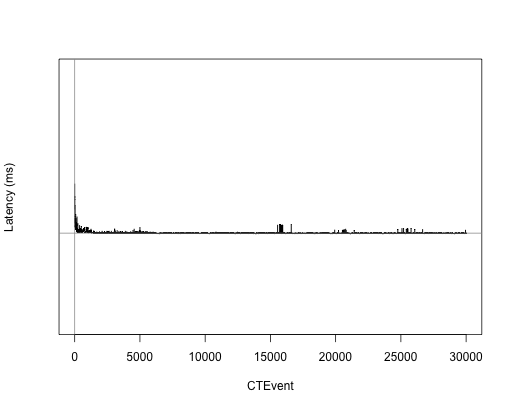
\includegraphics[width=\linewidth]{images/lat-log-graph/I11}
    				 \end{minipage}
    			   &	 \begin{minipage}{.15\textwidth}
     			 	
				\vspace{2pt}
     			 	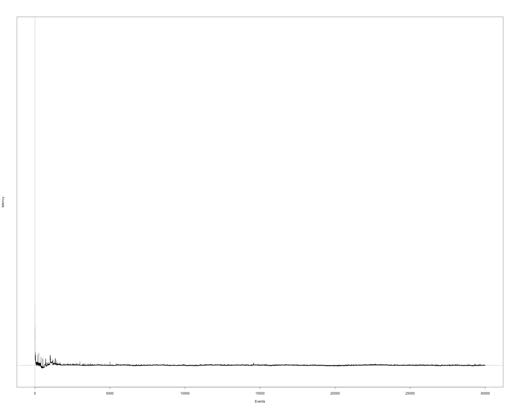
\includegraphics[width=\linewidth]{images/lat-log-graph/I13}
    				 \end{minipage}\\
		10000  &	 \begin{minipage}{.15\textwidth}
     			 	
				\vspace{2pt}
     			 	
\includegraphics[width=\linewidth]{images/lat-log-graph/I5}
    				 \end{minipage}
    			   &	 \begin{minipage}{.15\textwidth}
     			 	
				\vspace{2pt}
     			 	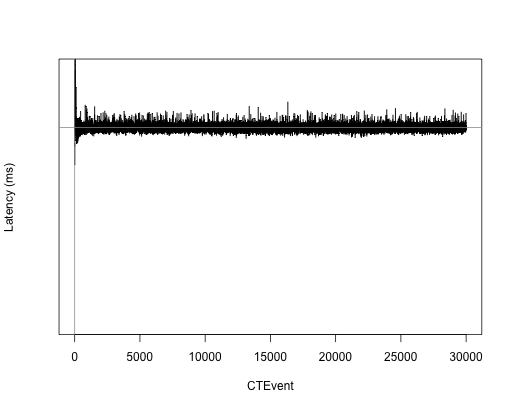
\includegraphics[width=\linewidth]{images/lat-log-graph/I9}
    				 \end{minipage}
    			   &	 \begin{minipage}{.15\textwidth}
     			 	
				\vspace{2pt}
     			 	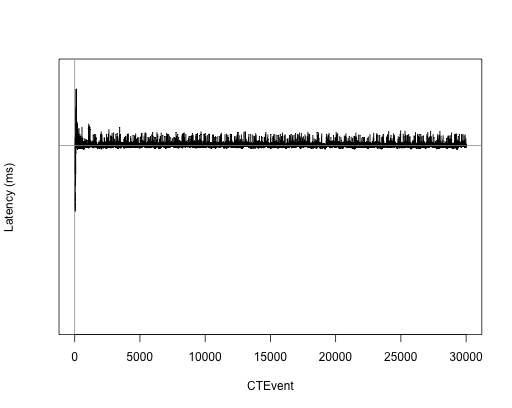
\includegraphics[width=\linewidth]{images/lat-log-graph/I12}
    				 \end{minipage}
    			   &	 \begin{minipage}{.15\textwidth}
     			 	
				\vspace{2pt}
     			 	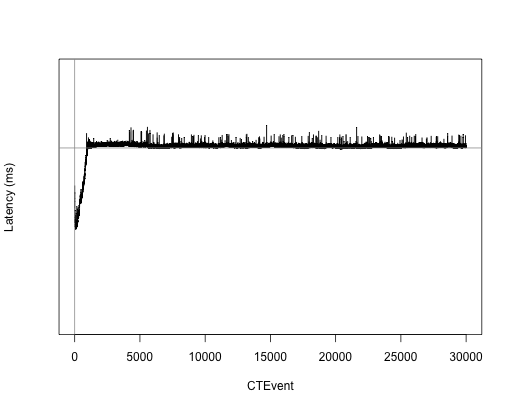
\includegraphics[width=\linewidth]{images/lat-log-graph/I14}
    				 \end{minipage}
    			   &	 \begin{minipage}{.15\textwidth}
     			 	
				\vspace{2pt}
     			 	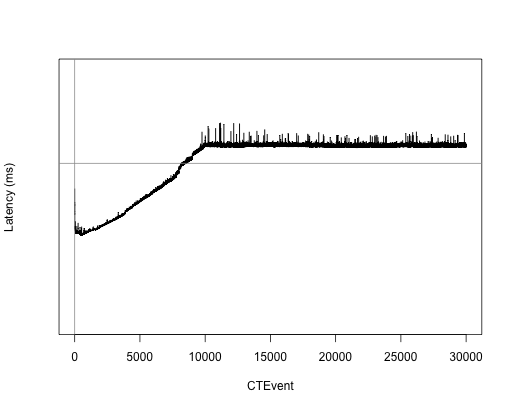
\includegraphics[width=\linewidth]{images/lat-log-graph/I15}
    				 \end{minipage}\\
		\hline % inserts single-line
	 \end{tabular}
	}
	\caption[\textsc{Analyser} Investigation Stack - Level 2 - Pattern Identification - Latency - Baselines GN and GI]{The figure shows the  representation in the time domain of latency for GN (a) and GI (b).} 
 	\label{tab:level2-latency-graph}
\end{table}

\begin{table}[htbp]
	\centering
	\scriptsize
	\subtable[Triple Naive]{%
		\begin{tabular}{l | ccccc} % creating eight columns
	  	\hline
		Triple  & \multicolumn{5}{c}{Slots}  \\
		in & \multicolumn{5}{c}{Number}  \\
		Window  & 1 & 10 & 100 & 1000&10000\\
		\hline
			\hline
		1	   &\begin{minipage}{.15\textwidth}
     			 	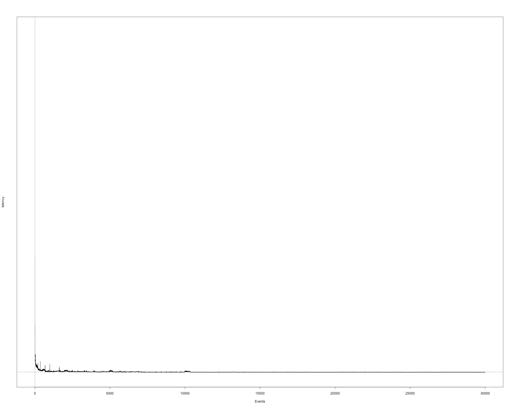
\includegraphics[width=\linewidth]{images/lat-log-triple/N1}
    				 \end{minipage}\\			
		10	   & \begin{minipage}{.15\textwidth}
     			 	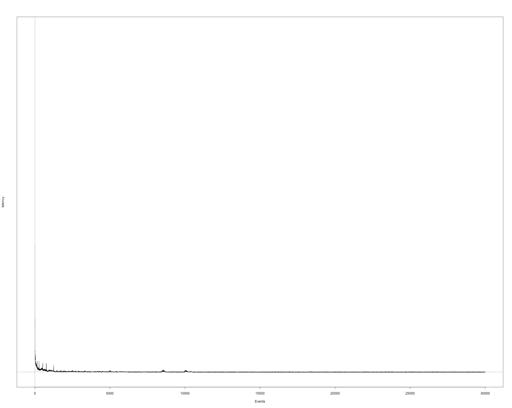
\includegraphics[width=\linewidth]{images/lat-log-triple/N2}
    				\end{minipage}
    			   & \begin{minipage}{.15\textwidth}
     			 	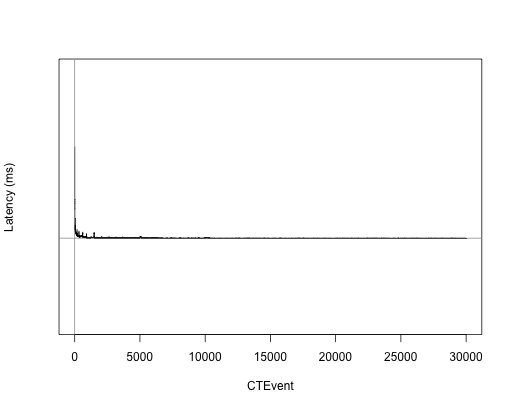
\includegraphics[width=\linewidth]{images/lat-log-triple/N6}
    				 \end{minipage}\\		
		100	   & \begin{minipage}{.15\textwidth}
     			 	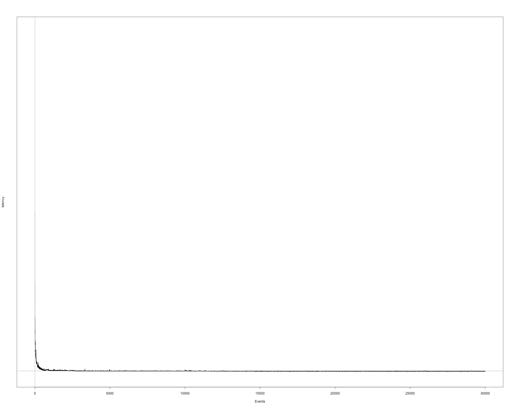
\includegraphics[width=\linewidth]{images/lat-log-triple/N3}
    				 \end{minipage}
    			   & \begin{minipage}{.15\textwidth}
     			 	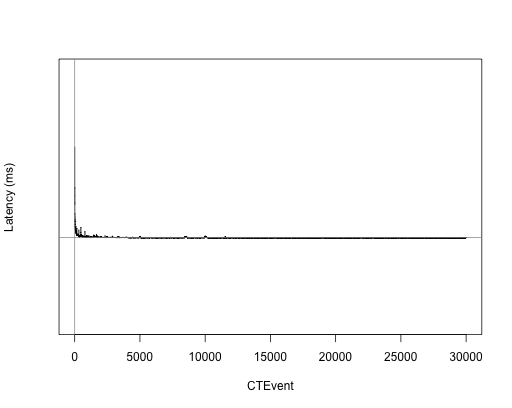
\includegraphics[width=\linewidth]{images/lat-log-triple/N7}
    				 \end{minipage}
    			   &	 \begin{minipage}{.15\textwidth}
     			 	\includegraphics[width=\linewidth]{images/lat-log-triple/N10}
    				 \end{minipage}\\	
		1000   &	 \begin{minipage}{.15\textwidth}
     			 	\includegraphics[width=\linewidth]{images/lat-log-triple/N4}
    				 \end{minipage}
    			   &	 \begin{minipage}{.15\textwidth}
     			 	\includegraphics[width=\linewidth]{images/lat-log-triple/N8}
    				 \end{minipage}
    			   &	 \begin{minipage}{.15\textwidth}
     			 	\includegraphics[width=\linewidth]{images/lat-log-triple/N11}
    				 \end{minipage}
    			   &	 \begin{minipage}{.15\textwidth}
     			 	\includegraphics[width=\linewidth]{images/lat-log-triple/N13}
    				 \end{minipage}\\
		10000  &	 \begin{minipage}{.15\textwidth}
     			 	\includegraphics[width=\linewidth]{images/lat-log-triple/N5}
    				 \end{minipage}
    			   &	 \begin{minipage}{.15\textwidth}
     			 	\includegraphics[width=\linewidth]{images/lat-log-triple/N9}
    				 \end{minipage}
    			   &	 \begin{minipage}{.15\textwidth}
     			 	\includegraphics[width=\linewidth]{images/lat-log-triple/N12}
    				 \end{minipage}
    			   &	 \begin{minipage}{.15\textwidth}
     			 	\includegraphics[width=\linewidth]{images/lat-log-triple/N14}
    				 \end{minipage}
    			   &	 \begin{minipage}{.15\textwidth}
     			 	\includegraphics[width=\linewidth]{images/lat-log-triple/N15}
    				 \end{minipage}\\
		\hline % inserts single-line
	 \end{tabular}
	}
	\subtable[Triple Incremental]{%
		\begin{tabular}{l | ccccc} % creating eight columns
	  	\hline
		Triple  & \multicolumn{5}{c}{Slots}  \\
		in & \multicolumn{5}{c}{Number}  \\
		Window  & 1 & 10 & 100 & 1000&10000\\
		\hline
			\hline
		1	   &\begin{minipage}{.15\textwidth}
     			 	\includegraphics[width=\linewidth]{images/lat-log-triple/I1}
    				 \end{minipage}\\			
		10	   & \begin{minipage}{.15\textwidth}
     			 	\includegraphics[width=\linewidth]{images/lat-log-triple/I2}
    				\end{minipage}
    			   & \begin{minipage}{.15\textwidth}
     			 	\includegraphics[width=\linewidth]{images/lat-log-triple/I6}
    				 \end{minipage}\\		
		100	   & \begin{minipage}{.15\textwidth}
     			 	\includegraphics[width=\linewidth]{images/lat-log-triple/I3}
    				 \end{minipage}
    			   & \begin{minipage}{.15\textwidth}
     			 	\includegraphics[width=\linewidth]{images/lat-log-triple/I7}
    				 \end{minipage}
    			   &	 \begin{minipage}{.15\textwidth}
     			 	\includegraphics[width=\linewidth]{images/lat-log-triple/I10}
    				 \end{minipage}\\	
		1000   &	 \begin{minipage}{.15\textwidth}
     			 	\includegraphics[width=\linewidth]{images/lat-log-triple/I4}
    				 \end{minipage}
    			   &	 \begin{minipage}{.15\textwidth}
     			 	\includegraphics[width=\linewidth]{images/lat-log-triple/I8}
    				 \end{minipage}
    			   &	 \begin{minipage}{.15\textwidth}
     			 	\includegraphics[width=\linewidth]{images/lat-log-triple/I11}
    				 \end{minipage}
    			   &	 \begin{minipage}{.15\textwidth}
     			 	\includegraphics[width=\linewidth]{images/lat-log-triple/I13}
    				 \end{minipage}\\
		10000  &	 \begin{minipage}{.15\textwidth}
     			 	\includegraphics[width=\linewidth]{images/lat-log-triple/I5}
    				 \end{minipage}
    			   &	 \begin{minipage}{.15\textwidth}
     			 	\includegraphics[width=\linewidth]{images/lat-log-triple/I9}
    				 \end{minipage}
    			   &	 \begin{minipage}{.15\textwidth}
     			 	\includegraphics[width=\linewidth]{images/lat-log-triple/I12}
    				 \end{minipage}
    			   &	 \begin{minipage}{.15\textwidth}
     			 	\includegraphics[width=\linewidth]{images/lat-log-triple/I14}
    				 \end{minipage}
    			   &	 \begin{minipage}{.15\textwidth}
     			 	\includegraphics[width=\linewidth]{images/lat-log-triple/I15}
    				 \end{minipage}\\
		\hline % inserts single-line
	 \end{tabular}
	}
	\caption[\textsc{Analyser} Investigation Stack - Level 2 - Pattern Identification - Latency - Baselines TN and TI]{The Linear Representation Scale of the Memory Time Series for TN and TI} 
 	\label{tab:level2-latency-triple}
	\end{table}

\begin{table}[htbp]
	\centering
	\scriptsize
	\subtable[Graph Naive]{%
		\begin{tabular}{l | ccccc} % creating eight columns
	  	\hline
		Triple  & \multicolumn{5}{c}{Slots}  \\
		in & \multicolumn{5}{c}{Number}  \\
		Window  & 1 & 10 & 100 & 1000&10000\\
		\hline
			\hline
		1	   &\begin{minipage}{.15\textwidth}
     			 	\includegraphics[width=\linewidth]{images/mema-graph/N1}
    				 \end{minipage}\\			
		10	   & \begin{minipage}{.15\textwidth}
     			 	\includegraphics[width=\linewidth]{images/mema-graph/N2}
    				\end{minipage}
    			   & \begin{minipage}{.15\textwidth}
     			 	\includegraphics[width=\linewidth]{images/mema-graph/N6}
    				 \end{minipage}\\		
		100	   & \begin{minipage}{.15\textwidth}
     			 	\includegraphics[width=\linewidth]{images/mema-graph/N3}
    				 \end{minipage}
    			   & \begin{minipage}{.15\textwidth}
     			 	\includegraphics[width=\linewidth]{images/mema-graph/N7}
    				 \end{minipage}
    			   &	 \begin{minipage}{.15\textwidth}
     			 	\includegraphics[width=\linewidth]{images/mema-graph/N10}
    				 \end{minipage}\\	
		1000   &	 \begin{minipage}{.15\textwidth}
     			 	\includegraphics[width=\linewidth]{images/mema-graph/N4}
    				 \end{minipage}
    			   &	 \begin{minipage}{.15\textwidth}
     			 	\includegraphics[width=\linewidth]{images/mema-graph/N8}
    				 \end{minipage}
    			   &	 \begin{minipage}{.15\textwidth}
     			 	\includegraphics[width=\linewidth]{images/mema-graph/N11}
    				 \end{minipage}
    			   &	 \begin{minipage}{.15\textwidth}
     			 	\includegraphics[width=\linewidth]{images/mema-graph/N13}
    				 \end{minipage}\\
		10000  &	 \begin{minipage}{.15\textwidth}
     			 	\includegraphics[width=\linewidth]{images/mema-graph/N5}
    				 \end{minipage}
    			   &	 \begin{minipage}{.15\textwidth}
     			 	\includegraphics[width=\linewidth]{images/mema-graph/N9}
    				 \end{minipage}
    			   &	 \begin{minipage}{.15\textwidth}
     			 	\includegraphics[width=\linewidth]{images/mema-graph/N12}
    				 \end{minipage}
    			   &	 \begin{minipage}{.15\textwidth}
     			 	\includegraphics[width=\linewidth]{images/mema-graph/N14}
    				 \end{minipage}
    			   &	 \begin{minipage}{.15\textwidth}
     			 	\includegraphics[width=\linewidth]{images/mema-graph/N15}
    				 \end{minipage}\\
		\hline % inserts single-line
	 \end{tabular}
	}
	\subtable[Graph Incremental]{%
		\begin{tabular}{l | ccccc} % creating eight columns
	  	\hline
		Triple  & \multicolumn{5}{c}{Slots}  \\
		in & \multicolumn{5}{c}{Number}  \\
		Window  & 1 & 10 & 100 & 1000&10000\\
		\hline
			\hline
		1	   &\begin{minipage}{.15\textwidth}
     			 	\includegraphics[width=\linewidth]{images/mema-graph/I1}
    				 \end{minipage}\\			
		10	   & \begin{minipage}{.15\textwidth}
     			 	\includegraphics[width=\linewidth]{images/mema-graph/I2}
    				\end{minipage}
    			   & \begin{minipage}{.15\textwidth}
     			 	\includegraphics[width=\linewidth]{images/mema-graph/I6}
    				 \end{minipage}\\		
		100	   & \begin{minipage}{.15\textwidth}
     			 	\includegraphics[width=\linewidth]{images/mema-graph/I3}
    				 \end{minipage}
    			   & \begin{minipage}{.15\textwidth}
     			 	\includegraphics[width=\linewidth]{images/mema-graph/I7}
    				 \end{minipage}
    			   &	 \begin{minipage}{.15\textwidth}
     			 	\includegraphics[width=\linewidth]{images/mema-graph/I10}
    				 \end{minipage}\\	
		1000   &	 \begin{minipage}{.15\textwidth}
     			 	\includegraphics[width=\linewidth]{images/mema-graph/I4}
    				 \end{minipage}
    			   &	 \begin{minipage}{.15\textwidth}
     			 	\includegraphics[width=\linewidth]{images/mema-graph/I8}
    				 \end{minipage}
    			   &	 \begin{minipage}{.15\textwidth}
     			 	\includegraphics[width=\linewidth]{images/mema-graph/I11}
    				 \end{minipage}
    			   &	 \begin{minipage}{.15\textwidth}
     			 	\includegraphics[width=\linewidth]{images/mema-graph/I13}
    				 \end{minipage}\\
		10000  &	 \begin{minipage}{.15\textwidth}
     			 	\includegraphics[width=\linewidth]{images/mema-graph/I5}
    				 \end{minipage}
    			   &	 \begin{minipage}{.15\textwidth}
     			 	\includegraphics[width=\linewidth]{images/mema-graph/I9}
    				 \end{minipage}
    			   &	 \begin{minipage}{.15\textwidth}
     			 	\includegraphics[width=\linewidth]{images/mema-graph/I12}
    				 \end{minipage}
    			   &	 \begin{minipage}{.15\textwidth}
     			 	\includegraphics[width=\linewidth]{images/mema-graph/I14}
    				 \end{minipage}
    			   &	 \begin{minipage}{.15\textwidth}
     			 	\includegraphics[width=\linewidth]{images/mema-graph/I15}
    				 \end{minipage}\\
		\hline % inserts single-line
	 \end{tabular}
	}
	\caption[\textsc{Analyser} Investigation Stack - Level 2 - Pattern Identification - Memory - Baselines GN and GI]{The Linear Representation Scale of the Memory Time Series for GN and GI} 
  	\label{tab:level2-memory-graph}
	\end{table}

\begin{table}[htbp]
	\centering
	\scriptsize
	\subtable[Triple Naive]{%
		\begin{tabular}{l | ccccc} % creating eight columns
	  	\hline
		Triple  & \multicolumn{5}{c}{Slots}  \\
		in & \multicolumn{5}{c}{Number}  \\
		Window  & 1 & 10 & 100 & 1000&10000\\
		\hline
			\hline
		1	   &\begin{minipage}{.15\textwidth}
     			 	\includegraphics[width=\linewidth]{images/mema-triple/N1}
    				 \end{minipage}\\			
		10	   & \begin{minipage}{.15\textwidth}
     			 	\includegraphics[width=\linewidth]{images/mema-triple/N2}
    				\end{minipage}
    			   & \begin{minipage}{.15\textwidth}
     			 	\includegraphics[width=\linewidth]{images/mema-triple/N6}
    				 \end{minipage}\\		
		100	   & \begin{minipage}{.15\textwidth}
     			 	\includegraphics[width=\linewidth]{images/mema-triple/N3}
    				 \end{minipage}
    			   & \begin{minipage}{.15\textwidth}
     			 	\includegraphics[width=\linewidth]{images/mema-triple/N7}
    				 \end{minipage}
    			   &	 \begin{minipage}{.15\textwidth}
     			 	\includegraphics[width=\linewidth]{images/mema-triple/N10}
    				 \end{minipage}\\	
		1000   &	 \begin{minipage}{.15\textwidth}
     			 	\includegraphics[width=\linewidth]{images/mema-triple/N4}
    				 \end{minipage}
    			   &	 \begin{minipage}{.15\textwidth}
     			 	\includegraphics[width=\linewidth]{images/mema-triple/N8}
    				 \end{minipage}
    			   &	 \begin{minipage}{.15\textwidth}
     			 	\includegraphics[width=\linewidth]{images/mema-triple/N11}
    				 \end{minipage}
    			   &	 \begin{minipage}{.15\textwidth}
     			 	\includegraphics[width=\linewidth]{images/mema-triple/N13}
    				 \end{minipage}\\
		10000  &	 \begin{minipage}{.15\textwidth}
     			 	\includegraphics[width=\linewidth]{images/mema-triple/N5}
    				 \end{minipage}
    			   &	 \begin{minipage}{.15\textwidth}
     			 	\includegraphics[width=\linewidth]{images/mema-triple/N9}
    				 \end{minipage}
    			   &	 \begin{minipage}{.15\textwidth}
     			 	\includegraphics[width=\linewidth]{images/mema-triple/N12}
    				 \end{minipage}
    			   &	 \begin{minipage}{.15\textwidth}
     			 	\includegraphics[width=\linewidth]{images/mema-triple/N14}
    				 \end{minipage}
    			   &	 \begin{minipage}{.15\textwidth}
     			 	\includegraphics[width=\linewidth]{images/mema-triple/N15}
    				 \end{minipage}\\
		\hline % inserts single-line
	 \end{tabular}
	}
	\subtable[Triple Incremental]{%
		\begin{tabular}{l | ccccc} % creating eight columns
	  	\hline
		Triple  & \multicolumn{5}{c}{Slots}  \\
		in & \multicolumn{5}{c}{Number}  \\
		Window  & 1 & 10 & 100 & 1000&10000\\
		\hline
			\hline
		1	   &\begin{minipage}{.15\textwidth}
     			 	\includegraphics[width=\linewidth]{images/mema-triple/I1}
    				 \end{minipage}\\			
		10	   & \begin{minipage}{.15\textwidth}
     			 	\includegraphics[width=\linewidth]{images/mema-triple/I2}
    				\end{minipage}
    			   & \begin{minipage}{.15\textwidth}
     			 	\includegraphics[width=\linewidth]{images/mema-triple/I6}
    				 \end{minipage}\\		
		100	   & \begin{minipage}{.15\textwidth}
     			 	\includegraphics[width=\linewidth]{images/mema-triple/I3}
    				 \end{minipage}
    			   & \begin{minipage}{.15\textwidth}
     			 	\includegraphics[width=\linewidth]{images/mema-triple/I7}
    				 \end{minipage}
    			   &	 \begin{minipage}{.15\textwidth}
     			 	\includegraphics[width=\linewidth]{images/mema-triple/I10}
    				 \end{minipage}\\	
		1000   &	 \begin{minipage}{.15\textwidth}
     			 	\includegraphics[width=\linewidth]{images/mema-triple/I4}
    				 \end{minipage}
    			   &	 \begin{minipage}{.15\textwidth}
     			 	\includegraphics[width=\linewidth]{images/mema-triple/I8}
    				 \end{minipage}
    			   &	 \begin{minipage}{.15\textwidth}
     			 	\includegraphics[width=\linewidth]{images/mema-triple/I11}
    				 \end{minipage}
    			   &	 \begin{minipage}{.15\textwidth}
     			 	\includegraphics[width=\linewidth]{images/mema-triple/I13}
    				 \end{minipage}\\
		10000  &	 \begin{minipage}{.15\textwidth}
     			 	\includegraphics[width=\linewidth]{images/mema-triple/I5}
    				 \end{minipage}
    			   &	 \begin{minipage}{.15\textwidth}
     			 	\includegraphics[width=\linewidth]{images/mema-triple/I9}
    				 \end{minipage}
    			   &	 \begin{minipage}{.15\textwidth}
     			 	\includegraphics[width=\linewidth]{images/mema-triple/I12}
    				 \end{minipage}
    			   &	 \begin{minipage}{.15\textwidth}
     			 	\includegraphics[width=\linewidth]{images/mema-triple/I14}
    				 \end{minipage}
    			   &	 \begin{minipage}{.15\textwidth}
     			 	\includegraphics[width=\linewidth]{images/mema-triple/I15}
    				 \end{minipage}\\
		\hline % inserts single-line
	 \end{tabular}
	}
	\caption[\textsc{Analyser} Investigation Stack - Level 2 - Pattern Identification - Memory - Baselines TN and NI]{The figure shows the  representation in the time domain of memory for TN (a) and TI (b)} 
 	\label{tab:level2-memory-triple}
\end{table}

\begin{table}[htbp]
	\centering
	\scriptsize
	\subtable[Graph Naive]{%
		\begin{tabular}{l | ccccc} % creating eight columns
	  	\hline
		Triple  & \multicolumn{5}{c}{Slots}  \\
		in & \multicolumn{5}{c}{Number}  \\
		Window  & 1 & 10 & 100 & 1000&10000\\
		\hline
			\hline
		1	   &\begin{minipage}{.15\textwidth}
     			 	\includegraphics[width=\linewidth]{images/mema-dens-graph/N1}
    				 \end{minipage}\\			
		10	   & \begin{minipage}{.15\textwidth}
     			 	\includegraphics[width=\linewidth]{images/mema-dens-graph/N2}
    				\end{minipage}
    			   & \begin{minipage}{.15\textwidth}
     			 	\includegraphics[width=\linewidth]{images/mema-dens-graph/N6}
    				 \end{minipage}\\		
		100	   & \begin{minipage}{.15\textwidth}
     			 	\includegraphics[width=\linewidth]{images/mema-dens-graph/N3}
    				 \end{minipage}
    			   & \begin{minipage}{.15\textwidth}
     			 	\includegraphics[width=\linewidth]{images/mema-dens-graph/N7}
    				 \end{minipage}
    			   &	 \begin{minipage}{.15\textwidth}
     			 	\includegraphics[width=\linewidth]{images/mema-dens-graph/N10}
    				 \end{minipage}\\	
		1000   &	 \begin{minipage}{.15\textwidth}
     			 	\includegraphics[width=\linewidth]{images/mema-dens-graph/N4}
    				 \end{minipage}
    			   &	 \begin{minipage}{.15\textwidth}
     			 	\includegraphics[width=\linewidth]{images/mema-dens-graph/N8}
    				 \end{minipage}
    			   &	 \begin{minipage}{.15\textwidth}
     			 	\includegraphics[width=\linewidth]{images/mema-dens-graph/N11}
    				 \end{minipage}
    			   &	 \begin{minipage}{.15\textwidth}
     			 	\includegraphics[width=\linewidth]{images/mema-dens-graph/N13}
    				 \end{minipage}\\
		10000  &	 \begin{minipage}{.15\textwidth}
     			 	\includegraphics[width=\linewidth]{images/mema-dens-graph/N5}
    				 \end{minipage}
    			   &	 \begin{minipage}{.15\textwidth}
     			 	\includegraphics[width=\linewidth]{images/mema-dens-graph/N9}
    				 \end{minipage}
    			   &	 \begin{minipage}{.15\textwidth}
     			 	\includegraphics[width=\linewidth]{images/mema-dens-graph/N12}
    				 \end{minipage}
    			   &	 \begin{minipage}{.15\textwidth}
     			 	\includegraphics[width=\linewidth]{images/mema-dens-graph/N14}
    				 \end{minipage}
    			   &	 \begin{minipage}{.15\textwidth}
     			 	\includegraphics[width=\linewidth]{images/mema-dens-graph/N15}
    				 \end{minipage}\\
		\hline % inserts single-line
	 \end{tabular}
	}
	\subtable[Graph Incremental]{%
		\begin{tabular}{l | ccccc} % creating eight columns
	  	\hline
		Triple  & \multicolumn{5}{c}{Slots}  \\
		in & \multicolumn{5}{c}{Number}  \\
		Window  & 1 & 10 & 100 & 1000&10000\\
		\hline
			\hline
		1	   &\begin{minipage}{.15\textwidth}
     			 	\includegraphics[width=\linewidth]{images/mema-dens-graph/I1}
    				 \end{minipage}\\			
		10	   & \begin{minipage}{.15\textwidth}
     			 	\includegraphics[width=\linewidth]{images/mema-dens-graph/I2}
    				\end{minipage}
    			   & \begin{minipage}{.15\textwidth}
     			 	\includegraphics[width=\linewidth]{images/mema-dens-graph/I6}
    				 \end{minipage}\\		
		100	   & \begin{minipage}{.15\textwidth}
     			 	\includegraphics[width=\linewidth]{images/mema-dens-graph/I3}
    				 \end{minipage}
    			   & \begin{minipage}{.15\textwidth}
     			 	\includegraphics[width=\linewidth]{images/mema-dens-graph/I7}
    				 \end{minipage}
    			   &	 \begin{minipage}{.15\textwidth}
     			 	\includegraphics[width=\linewidth]{images/mema-dens-graph/I10}
    				 \end{minipage}\\	
		1000   &	 \begin{minipage}{.15\textwidth}
     			 	\includegraphics[width=\linewidth]{images/mema-dens-graph/I4}
    				 \end{minipage}
    			   &	 \begin{minipage}{.15\textwidth}
     			 	\includegraphics[width=\linewidth]{images/mema-dens-graph/I8}
    				 \end{minipage}
    			   &	 \begin{minipage}{.15\textwidth}
     			 	\includegraphics[width=\linewidth]{images/mema-dens-graph/I11}
    				 \end{minipage}
    			   &	 \begin{minipage}{.15\textwidth}
     			 	\includegraphics[width=\linewidth]{images/mema-dens-graph/I13}
    				 \end{minipage}\\
		10000  &	 \begin{minipage}{.15\textwidth}
     			 	\includegraphics[width=\linewidth]{images/mema-dens-graph/I5}
    				 \end{minipage}
    			   &	 \begin{minipage}{.15\textwidth}
     			 	\includegraphics[width=\linewidth]{images/mema-dens-graph/I9}
    				 \end{minipage}
    			   &	 \begin{minipage}{.15\textwidth}
     			 	\includegraphics[width=\linewidth]{images/mema-dens-graph/I12}
    				 \end{minipage}
    			   &	 \begin{minipage}{.15\textwidth}
     			 	\includegraphics[width=\linewidth]{images/mema-dens-graph/I14}
    				 \end{minipage}
    			   &	 \begin{minipage}{.15\textwidth}
     			 	\includegraphics[width=\linewidth]{images/mema-dens-graph/I15}
    				 \end{minipage}\\
		\hline % inserts single-line
	 \end{tabular}
	}
	\caption[\textsc{Analyser} Investigation Stack - Level 2 - Pattern Identification - Memory Distribution - Baselines GN and GI]{GN and GI Distribution of Memory Time Series Values over 10 Intervals between the Minimum to the Maximum over all the Experiments} 
	\label{tab:level2-memory-density-graph}
	\end{table}

\begin{table}[htbp]
	\centering
	\scriptsize
	\subtable[Triple Naive]{%
		\begin{tabular}{l | ccccc} % creating eight columns
	 \hline
		\hline
		Triple  & \multicolumn{5}{c}{Slots}  \\
		in & \multicolumn{5}{c}{Number}  \\
		Window  & 1 & 10 & 100 & 1000&10000\\
		\hline
		1	   &\begin{minipage}{.15\textwidth}
     			 	\includegraphics[width=\linewidth]{images/mema-dens-triple/N1}
    				 \end{minipage}\\			
		10	   & \begin{minipage}{.15\textwidth}
     			 	\includegraphics[width=\linewidth]{images/mema-dens-triple/N2}
    				\end{minipage}
    			   & \begin{minipage}{.15\textwidth}
     			 	\includegraphics[width=\linewidth]{images/mema-dens-triple/N6}
    				 \end{minipage}\\		
		100	   & \begin{minipage}{.15\textwidth}
     			 	\includegraphics[width=\linewidth]{images/mema-dens-triple/N3}
    				 \end{minipage}
    			   & \begin{minipage}{.15\textwidth}
     			 	\includegraphics[width=\linewidth]{images/mema-dens-triple/N7}
    				 \end{minipage}
    			   &	 \begin{minipage}{.15\textwidth}
     			 	\includegraphics[width=\linewidth]{images/mema-dens-triple/N10}
    				 \end{minipage}\\	
		1000   &	 \begin{minipage}{.15\textwidth}
     			 	\includegraphics[width=\linewidth]{images/mema-dens-triple/N4}
    				 \end{minipage}
    			   &	 \begin{minipage}{.15\textwidth}
     			 	\includegraphics[width=\linewidth]{images/mema-dens-triple/N8}
    				 \end{minipage}
    			   &	 \begin{minipage}{.15\textwidth}
     			 	\includegraphics[width=\linewidth]{images/mema-dens-triple/N11}
    				 \end{minipage}
    			   &	 \begin{minipage}{.15\textwidth}
     			 	\includegraphics[width=\linewidth]{images/mema-dens-triple/N13}
    				 \end{minipage}\\
		10000  &	 \begin{minipage}{.15\textwidth}
     			 	\includegraphics[width=\linewidth]{images/mema-dens-triple/N5}
    				 \end{minipage}
    			   &	 \begin{minipage}{.15\textwidth}
     			 	\includegraphics[width=\linewidth]{images/mema-dens-triple/N9}
    				 \end{minipage}
    			   &	 \begin{minipage}{.15\textwidth}
     			 	\includegraphics[width=\linewidth]{images/mema-dens-triple/N12}
    				 \end{minipage}
    			   &	 \begin{minipage}{.15\textwidth}
     			 	\includegraphics[width=\linewidth]{images/mema-dens-triple/N14}
    				 \end{minipage}
    			   &	 \begin{minipage}{.15\textwidth}
     			 	\includegraphics[width=\linewidth]{images/mema-dens-triple/N15}
    				 \end{minipage}\\
		\hline % inserts single-line
	 \end{tabular}
	}
	\subtable[Triple Incremental]{%
		\begin{tabular}{l | ccccc} % creating eight columns
	  	\hline
					\hline
		Triple  & \multicolumn{5}{c}{Slots}  \\
		in & \multicolumn{5}{c}{Number}  \\
		Window  & 1 & 10 & 100 & 1000&10000\\
		\hline
		1	   &\begin{minipage}{.15\textwidth}
     			 	\includegraphics[width=\linewidth]{images/mema-dens-triple/I1}
    				 \end{minipage}\\			
		10	   & \begin{minipage}{.15\textwidth}
     			 	\includegraphics[width=\linewidth]{images/mema-dens-triple/I2}
    				\end{minipage}
    			   & \begin{minipage}{.15\textwidth}
     			 	\includegraphics[width=\linewidth]{images/mema-dens-triple/I6}
    				 \end{minipage}\\		
		100	   & \begin{minipage}{.15\textwidth}
     			 	\includegraphics[width=\linewidth]{images/mema-dens-triple/I3}
    				 \end{minipage}
    			   & \begin{minipage}{.15\textwidth}
     			 	\includegraphics[width=\linewidth]{images/mema-dens-triple/I7}
    				 \end{minipage}
    			   &	 \begin{minipage}{.15\textwidth}
     			 	\includegraphics[width=\linewidth]{images/mema-dens-triple/I10}
    				 \end{minipage}\\	
		1000   &	 \begin{minipage}{.15\textwidth}
     			 	\includegraphics[width=\linewidth]{images/mema-dens-triple/I4}
    				 \end{minipage}
    			   &	 \begin{minipage}{.15\textwidth}
     			 	\includegraphics[width=\linewidth]{images/mema-dens-triple/I8}
    				 \end{minipage}
    			   &	 \begin{minipage}{.15\textwidth}
     			 	\includegraphics[width=\linewidth]{images/mema-dens-triple/I11}
    				 \end{minipage}
    			   &	 \begin{minipage}{.15\textwidth}
     			 	\includegraphics[width=\linewidth]{images/mema-dens-triple/I13}
    				 \end{minipage}\\
		10000  &	 \begin{minipage}{.15\textwidth}
     			 	\includegraphics[width=\linewidth]{images/mema-dens-triple/I5}
    				 \end{minipage}
    			   &	 \begin{minipage}{.15\textwidth}
     			 	\includegraphics[width=\linewidth]{images/mema-dens-triple/I9}
    				 \end{minipage}
    			   &	 \begin{minipage}{.15\textwidth}
     			 	\includegraphics[width=\linewidth]{images/mema-dens-triple/I12}
    				 \end{minipage}
    			   &	 \begin{minipage}{.15\textwidth}
     			 	\includegraphics[width=\linewidth]{images/mema-dens-triple/I14}
    				 \end{minipage}
    			   &	 \begin{minipage}{.15\textwidth}
     			 	\includegraphics[width=\linewidth]{images/mema-dens-triple/I15}
    				 \end{minipage}\\
		\hline % inserts single-line
	 \end{tabular}
	}
	\caption[\textsc{Analyser} Investigation Stack - Level 2 - Pattern Identification - Memory Distribution - Baselines TN and TI]{	Figure shows how memory values for TN (a) and TI (b) are distributed over ten intervals between the global  minimum and maximum of all the SOAK tests results}�
	\label{tab:level2-memory-density-triple}
	\end{table}

\begin{figure}[tbhp]
  \centering
  \subfigure[GN Exp 11, \textsc{CTEvent} Size = 10 Num.Slot = 100]{\includegraphics[width=\linewidth]{images/level3-not-steady-naive-graph-en11}}
  \subfigure[TI Exp 11, \textsc{CTEvent} Size = 10 Num.Slot = 100]{\includegraphics[width=\linewidth]{images/level3-not-steady-inc-stmt-en11}}
  \caption[\textsc{Analyser} Investigation Stack - Level 3 - Intra Experiment Comparison - SOAK Test Latency vs Memory Not Steady State Reaching]{Comparison between memory and latency on difference in Steady State condition reaching} 
  \label{fig:level3-not-steady-naive-graph-en11}
\end{figure}

\begin{figure}[tbph]
  \centering
  \subfigure[GN Exp 7, \textsc{CTEvent} Size = 10, Num.Slot = 10]{\includegraphics[width=\linewidth]{images/level3-steady-naive-graph-en7}}
   \subfigure[GI Exp 12, \textsc{CTEvent} Size = 100, Num.Slot = 100]{\includegraphics[width=\linewidth]{images/level3-steady-inc-graph-en12}}
  	\caption[\textsc{Analyser} Investigation Stack - Level 3 - Intra Experiment Comparison - SOAK Test Latency vs Memory Steady State Reaching]{Comparison of steady state condition reaching between latency and memory}
  	\label{fig:level3-steady-naive-graph-en12-7}  	
\end{figure}

\begin{figure}[tbph]
  \centering
  \subfigure[TN Exp 15, \textsc{CTEvent} Size = 1 Num.Slot = 10000]{
	\includegraphics[width=\linewidth]{images/level3-filling-naive-stmt-en15}
	}
\subfigure[TI Exp 15, \textsc{CTEvent} Size = 1 Num.Slot = 10000]{
	\includegraphics[width=\linewidth]{images/level3-filling-inc-stmt-en15}
	}
	\caption[\textsc{Analyser} Investigation Stack - Level 3 - Intra Experiment Comparison - SOAK Test Latency vs Memory Filling Phenomena]{Comparison of filling phenomena between latency and memory} 
  	\label{fig:level3-filling-inc-stmt-en15}
\end{figure}

\pagebreak

\section{Step Response Test Evaluation Results}\label{sec:stressres}

In the previous sections of this chapter we presented the three contributes that \name provides to the SR research: (i) we explain how to design experiments through the \name definition $<\mathcal{E},\mathcal{D},\mathcal{T},\mathcal{Q}>$ (Section~\ref{sec:experiment-design}); (ii) we include two examples of test sets and the lecture-key to drive the result analysis for one of them (Section~\ref{sec:experiment-setup}); (iii) we provide a concrete use-case analysis, exploiting one of the test set provided in (ii) (Section~\ref{sec:soakres}). However, in other to prove that \name supports the SCRA we are still missing a forth contribution: (iv) proving the generality of (i), (ii), (iii) and consequently demonstrate the flexibility of the research powered by \namens.

Further examples of (i), (ii) and (iii) are not enough to show \name capabilities proving (iv). We have to change the research paradigm, providing a complete different kind of analysis. SOAK Testing is a standard testing procedure for dynamic systems (see Section~\ref{sec:software-testing}) and Step Response Testing is a standard complementary procedure for it. In order to prove the generality of the SCRA enabled by \namens, we provide an example of \textit{Inter Experiment} analysis. We exploit the Step Response Test set presented in Section~\ref{sec:step-es} together with the results of the SOAK Test set of Section~\ref{sec:soak-es}, presenting a new kind of insight.

In the following we briefly show the Step Response testing results, exploiting the \textsc{Analyser} Investigation Stack, except for Level 2 as we explain in Section~\ref{sec:level2-step-pattern}. We focus on the evaluation, because further details of each level of the Investigation Stack can be found in Section~\ref{sec:analyser} and Section~\ref{sec:analyser-impl}, while the design of this experimental set is described in Section~\ref{sec:step-es}.

\subsection{Steady State Identification Block}\label{sec:level0-step-ssib}

The analysis starts with the identification of the Steady State condition for the variables involved in the experiments, memory and latency, as we did in Section~\ref{sec:level0-step-ssib}. For SOAK Test experiments the Steady State condition has a single meaning w.r.t the execution. Instead, for Step Response Test experiments we can identify two possible Steady State conditions: ante step (AS) and post step (PS). In this section, we apply a different comparative approach, contrasting the results of Step Response and SOAK experiment, which are relate as reported in Section~\ref{sec:step-es}. 

The SSI block analysis is extended to reach this experimental characteristic. Tables~\ref{tab:ss-step-latency} and~\ref{tab:ss-step-memory} report the results from the SSI block. Each of them includes the results for the two phases which compose a Step Response Test: ante-step (AS) and post-step (PS). 

As we expected, latency reaches Steady State condition for both the AS and the PS phases in all experiments. Instead memory does not reach the Steady State condition for several experiments,  which are highlighted in Table~\ref{tab:ss-step-memory}, and independently from AS and PS phases.

\begin{table}[h]
\centering
\scriptsize
\begin{tabular}{ll|c|c|c|c|c|c|c|c}
\hline
\textsc{CTEvent}&\textsc{CTEvent}&\multicolumn{2}{c|}{GN}& \multicolumn{2}{c|}{GI}& \multicolumn{2}{c|}{TN}& \multicolumn{2}{c}{TI} \\
 Init Size & Final Size & AS& PS& AS& PS& AS& PS& AS & PS\\ 
\hline
\hline
10 & 100 & Yes& Yes & Yes & Yes & Yes& Yes & Yes & Yes \\ 
10 & 1000& Yes& Yes& Yes & Yes& Yes& Yes& Yes& Yes\\ 
100& 1000& Yes & Yes& Yes & Yes& Yes & Yes& Yes  & Yes\\ 
\hline
\end{tabular}
\caption[Steady State Identification Block - Step Response Summary Table - Latency]{Steady State Identification Block - Step Response Summary Table - The Steady State condition is evaluated for both the two phases of the Step Response Test execution: Ante Step (AS) and Post Step (PS). This tables report the SSI block results for the evaluation of the latency variable. All the experiment reach the Steady State for both the AS and the PS phases.}
\label{tab:ss-step-latency}
\end{table}


\begin{table}[h]
\centering
\scriptsize
\begin{tabular}{ll|c|c|c|c|c|c|c|c}
\hline
\textsc{CTEvent}&\textsc{CTEvent}&\multicolumn{2}{c|}{GN}& \multicolumn{2}{c|}{GI}& \multicolumn{2}{c|}{TN}& \multicolumn{2}{c}{TI} \\
 Init Size & Final Size & AS& PS& AS& PS& AS& PS& AS & PS\\ 
\hline
\hline
10 & 100 & Yes& \cellcolor[HTML]{C0C0C0}No & \cellcolor[HTML]{C0C0C0}No & \cellcolor[HTML]{C0C0C0}No & Yes& \cellcolor[HTML]{C0C0C0}No & \cellcolor[HTML]{FFFFFF}Yes & \cellcolor[HTML]{C0C0C0}No \\ 
10 & 1000& Yes& Yes& \cellcolor[HTML]{C0C0C0}No & Yes& Yes& Yes& Yes& Yes\\ 
100& 1000& \cellcolor[HTML]{C0C0C0}No & Yes& \cellcolor[HTML]{C0C0C0}No & Yes& \cellcolor[HTML]{C0C0C0}No & Yes& \cellcolor[HTML]{C0C0C0}No  & Yes\\ 
\hline
\end{tabular}
\caption[Steady State Identification Block - Step Response Summary Table - Memory]{Steady State Identification Block - Step Response Summary Table - The Steady State condition is evaluated for both the two phases of the Step Response Test execution: Ante Step (AS) and Post Step (PS). This tables report the SSI block results for the evaluation of the memory variable. Several experiments, highlighted in the table, do not reach the Steady State in one or both the AS and the PS phases.}
\label{tab:ss-step-memory}
\end{table}

\subsection{Level 0 - Dashboard Views}\label{sec:level0-step-dashboard}

In this section, we continue the evaluation providing some examples of an easy-to-ready dashboard view. As we did Section~\ref{sec:soak-es} where we tried to identify a hierarchy between the tested solution (the Baselines). 

\begin{figure}[htbp]
	\centering
	\includegraphics[width=\linewidth]{images/level-0-step-dashboard-1}	
	\caption[\textsc{Analyser} Investigation Stack - Level 0 - Step Response Dashboard One]{\textsc{Analyser} Investigation Stack - Level 0 - Step Response Dashboard One - The figure shows in log-scale the average performance values for memory (Y) and latency (X) of the Step Response Test with an \textsc{CTEvent} Initial Size of 10 and with a \textsc{CTEvent} Final Size of 1000. We distinguish the two phases that compose the experiment as ante-step (AS) and post-step (PS) with different representation explained in the Legend}
	\label{fig:level-0-step-dashboard-1}
\end{figure}
\begin{figure}[htbp]
	\centering
	\includegraphics[width=0.90\linewidth]{images/level-0-step-dashboard-2}	
	\caption[\textsc{Analyser} Investigation Stack - Level 0 - Step Response Dashboard Two - Related SOAK Experiments]{
\textsc{Analyser} Investigation Stack - Level 0 - Step Response Dashboard Two - Related SOAK Experiments - The figure shows in log-scale the average performance values for memory (Y) and latency (X) of the SOAK Experiment related to the Step Test of Figure~\ref{fig:level-0-step-dashboard-1}. The SOAK test related to the first Step Response phase (SOAK I) has a \textsc{CTEvent} size of 10, while the SOAK test related to the second Step Response phase (SOAK F) has a \textsc{CTEvent} size of 1000.}
	\label{fig:level-0-step-dashboard-2}
\end{figure}

The Level 0 comparison is summarised in two separated dashboards: Figure~\ref{fig:level-0-step-dashboard-1} shows the two phases of the Step Response Test execution, AS and PS. Figure~\ref{fig:level-0-step-dashboard-2} displays the results of the relative SOAK experiments. Considering the figures, SOAK I and AS results refer to a \textsc{CTEvent} size of 10, while SOAK F and PS refer to a \textsc{CTEvent} size of 1000.

Observing the figures we can read an insight: the performances at Steady State for both the AS and PS phases are similar to the relative SOAK one. This means that the transitory phase does not influence the Steady State condition reached for this particular experiment.

\subsection{Level 1 - Statistical Values Comparison}\label{sec:level1-step-stats}

%Level 0 has proved that, for the studied case, the average result values are comparable. However we know from Section~\ref{sec:eval-level3} that the initial transitory phase of an RSP Engine is very different between memory and latency. Moreover, it may depend on the filling phenomena that may affect the window (This is not certainly the case of our naive experiment set).

In this section, we try to extend the statistical \textit{Inter Experiment} comparison proposed in Section~\ref{sec:eval-level1}. We provide a different layout, which allows to compare the Baseline performances between the two phases of the Step Response tests and the relative SOAK experiment results.

Tables from~\ref{tab:step_latency_comparisons_mean} and~\ref{tab:step_memory_comparisons_max} show the worsening of latency and memory values. We compare Step Response Test ante-step (AS) phase with the relative SOAK Test, named as SOAK I, and the Step Response post-step (PS) with the relative SOAK Test, named as SOAK F.  We exploit the quantitative approach of Level 1 to evidence the differences between the two experiment results.


Tables~\ref{tab:step_latency_comparisons_mean} and~\ref{tab:step_memory_comparisons_mean} confirm what we have seen in the dashboard views at Level 0. We can observe that for the average values the variations between AS and SOAK I and between PS and SOAK F are minimal, around the 0.5\%  with some outliers of 10-12\%. Exactly what the dashboards present in Figures~\ref{fig:level-0-step-dashboard-1} and~\ref{fig:level-0-step-dashboard-2}. 

Thus, the comparison of average data seems to be not so interesting. A better point of analysis is given by Tables~\ref{tab:step_latency_comparisons_max} and~\ref{tab:step_memory_comparisons_max}, which apply the same layout to the comparison of memory and latency maximum values. Notice that we take all the execution, considering also the initial transitory phase which usually contains the most high values.

We compare the maximum latency values for the Test SOAK I and SOAK F, observing that: (i) the differences between SOAK I and AS, which involved the Step Response test warm-up, follow the same behaviour and confirms the insight from Table~\ref{tab:step_latency_comparisons_mean}. (ii) The performance improvement between PS and SOAK F is much more relevant, always greater than 50\% and some over the 80\%. This insight points out that there is a initialisation cost that influences the performances, and it must be considered during the deployment of an RSP Engine. 

Table~\ref{tab:step_memory_comparisons_max} shows a different situation for memory. Nothing can be said about the comparison between SOAK I and Step Response AS except that the Step Response AS always consumes more memory w.r.t the SOAK I. Considering the comparison between Step Response PS and SOAK F, we cannot observe in general the same situation of Table Table~\ref{tab:step_latency_comparisons_max}, but a similar behaviour is present for Baselines GI and GN, which have a bigger increase in the Step Response PS than TN and TI.

\subsection{Level 2 - Pattern Identification}\label{sec:level2-step-pattern}

As we reported in the introduction, we actually do not apply this level analysis. The motivation can be found in the restricted dimension of the Step Response test set, which lacks the minimum amount of information to perform pattern identification step. Moreover the number of slots, which compose the active window, is fixed to ten for this experiment set. In general DSMSs do not allow to change the window dimension during the execution. This limitation makes even less interesting the pattern analysis, since we have only a single controlling variable.

\subsection{Level 3 - Single Visual Comparison}\label{sec:level3-step-inter}

Finally, we conclude the SOAK Testing analysis through several examples of \textit{Intra Experiment} comparison (see Section~\ref{sec:eval-level3}). In this section we provide the alternative analysis method of Level 3, presented in Section~\ref{sec:analyser}: the \textit{Inter Experiment} comparison method.

Figures~\ref{fig:level3-step} (a) and (b) draw, on the same graphl, the latency and the memory series for three experiments.  We build the comparison diversifying the \textit{CTEvent} size, since the number of slots is fixed to ten.
\pagebreak

Thus, the involved experiments are:
\begin{itemize}
\item Step Response Test with \textsc{CTEvent} initial size fixed to 10 Triples and Final Size fixed to 100 triples.
\item SOAK Test Number 7, with \textsc{CTEvent} size fixed to 10 Triples.
\item SOAK Test Number 8, with \textsc{CTEvent} size fixed to 100 Triples.
\end{itemize}

Notice that, Figure~\ref{fig:level3-step}.a reports the latency time series for the Baseline TI, while~\ref{fig:level3-step}.b presents the memory usage for the Baseline GI. We selected the two most expressive graphs, in order to show the following insight.

%The Figures~\ref{fig:level3-step} (a) and (b) answer two standard questions of Step Response Test, which ,contextualised in SR, are (Q.1) There is an initial transitory phase also for a sudden changes in the RDF Stream dimension, an thus in number of triple in the active window? (Q.2) Does the system reaches a Steady State condition after a sudden changes in the RDF Stream dimension, an thus in number of triple in the active window?
%
%An answer to Q.1 can be found in Figure~\ref{fig:level3-step}.a. It is possible to see that after the step there is no transitory phase for the RSP Engine latency. A similar behaviour is observable for memory in Figure~\ref{fig:level3-step}.b. 
%
%A positive answer to Q.2 is given by the Latency, whose Steady State condition reaching does not changes between the SOAK Tests and the Step Response phases AS and PS. For memory instead, the growth trend is still present  in both the SOAK and Step Response tests, but in tje second one Java anticipates its optimisation policies, limiting the variance of memory oscillations. 

In Figure~\ref{fig:level3-step}.a  it is possible to see that after the step there is no transitory phase for the RSP Engine latency. A similar behaviour is observable, for memory, in Figure~\ref{fig:level3-step}.b. About the Steady State condition, we can observe that latency behaviour does not changes if compare the SOAK Tests 7 and 8 with the relative  Step Response phases AS and PS. The insight is quite more complex for memory. The growth trend is still present in both the SOAK and Step Response tests, but in the second one Java anticipates its optimisation policies, limiting the variance of memory oscillations. 


\begin{figure}[tbh]
  \centering
  \subfigure[TI Step Response vs SOAK Tests - \textsc{CTEvent} Init Size = 10 Final Size 100 N.Slots = 10]{
	\includegraphics[width=\linewidth]{images/step_lat_incremental_triple_soak_init_7soak_final_8step_101}
	}
\subfigure[GI Step Response vs SOAK Tests - \textsc{CTEvent} Init Size = 10 Final Size 100 N.Slots = 10]{
	\includegraphics[width=\linewidth]{images/step_mema_incremental_graph_soak_init_7soak_final_8step_101}
	}
	\caption[\textsc{Analyser} Investigation Stack - Level 3 - Inter Experiment Comparison - Step Response Test]{\textsc{Analyser} Investigation Stack - Level 3 -  Inter Experiment comparisons of latency (Y) in  Figure (a) and memory (Y) in Figure (b) over the all the experiment execution \textsc{CTEvent} (X).} 
  	\label{fig:level3-step}
\end{figure}

%\begin{sidewaystable}
	\centering
	\scriptsize
	\begin{tabular}{c|c|cc|cc|cc|cc|} % creating eight columns
	  	\hline
		Init Size&FinalSize &\multicolumn{2}{c}{Graph Naive}  &\multicolumn{2}{c}{Triple Naive}&\multicolumn{2}{c}{Graph Inc}  &\multicolumn{2}{c}{Triple Inc}\\\
		&& SOAK Init & SOAK Final& SOAK Init & SOAK Final& SOAK Init & SOAK Final& SOAK Init & SOAK Final\\
		\hline
		\hline
		10&100&0,83\%&	-2,36\%&	1,29\%&	-1,44\%&	2,07\%&	-0,94\%&	-0,12\%&	0,49\%\\	
		10&1000&0,98\%&	-0,33\%&	1,77\%&	-0,07\%&	1,71\%&	0,98\%&	-0,12\%&	0,56\%\\
	
		100&100&	-0,47\%&	-1,18\%&	0,68\%&	0,00\%&	0,92\%&	1,05\%&	1,51\%&	-0,16\%\\
		\hline % inserts single-line
	\end{tabular}
	\caption[\textsc{Analyser} Investigation Stack - Level 1 - SOAK Test Average Latency Comparison]{Mean Latency Comparison Step Response}

	\label{tab:soak_latency_comparisons}	

	\centering
	\scriptsize
	\begin{tabular}{c|c|cc|cc|cc|cc|} % creating eight columns
	  	\hline
		Init Size&FinalSize &\multicolumn{2}{c}{Graph Naive}  &\multicolumn{2}{c}{Triple Naive}&\multicolumn{2}{c}{Graph Inc}  &\multicolumn{2}{c}{Triple Inc}\\\
		&& SOAK Init & SOAK Final& SOAK Init & SOAK Final& SOAK Init & SOAK Final& SOAK Init & SOAK Final\\
		\hline
		\hline
		10	&100	&4,02\%&	-661,17\%&	8,10\%&	-773,91\%&	2,07\%&	-1100,97\%&	2,94\%&	-1136,63\%\\	
		10	&1000	&3,05\%&	-102,62\%&	12,95\%&	-120,48\%&	1,71\%&	-122,80\%&	1,78\%&	-161,61\%	\\
		100	&1000&	1,38\%&	-106,32\%&	6,20\%&	-137,48\%&	0,92\%&	-116,47\%&	2,35\%&	-155,82\%	\\

		\hline % inserts single-line
	\end{tabular}
	\caption[\textsc{Analyser} Investigation Stack - Level 1 - SOAK Test Average Latency Comparison]{Max Latency Comparison Step Response}

	\label{tab:soak_latency_comparisons}	
\end{sidewaystable}

\begin{sidewaystable}
	\centering
	\scriptsize
	\begin{tabular}{c|c|cc|cc|cc|cc|} % creating eight columns
	  	\hline
		Init Size&FinalSize &\multicolumn{2}{c}{Graph Naive}  &\multicolumn{2}{c}{Triple Naive}&\multicolumn{2}{c}{Graph Inc}  &\multicolumn{2}{c}{Triple Inc}\\\
		&& SOAK Init & SOAK Final& SOAK Init & SOAK Final& SOAK Init & SOAK Final& SOAK Init & SOAK Final\\
		\hline
		\hline
		10&100&0,83\%&	-2,36\%&	1,29\%&	-1,44\%&	2,07\%&	-0,94\%&	-0,12\%&	0,49\%\\	
		10&1000&0,98\%&	-0,33\%&	1,77\%&	-0,07\%&	1,71\%&	0,98\%&	-0,12\%&	0,56\%\\
	
		100&100&	-0,47\%&	-1,18\%&	0,68\%&	0,00\%&	0,92\%&	1,05\%&	1,51\%&	-0,16\%\\
		\hline % inserts single-line
	\end{tabular}
	\caption[\textsc{Analyser} Investigation Stack - Level 1 - SOAK Test Average Latency Comparison]{Mean Latency Comparison Step Response}
	\label{tab:step_latency_comparisons_mean}	

	\begin{tabular}{c|c|cc|cc|cc|cc|} % creating eight columns
	  	\hline
		Init Size&FinalSize &\multicolumn{2}{c}{Graph Naive}  &\multicolumn{2}{c}{Triple Naive}&\multicolumn{2}{c}{Graph Inc}  &\multicolumn{2}{c}{Triple Inc}\\\
		&& SOAK Init & SOAK Final& SOAK Init & SOAK Final& SOAK Init & SOAK Final& SOAK Init & SOAK Final\\
		\hline
		\hline
		10	&100	&4,02\%&	-661,17\%&	8,10\%&	-773,91\%&	2,07\%&	-1100,97\%&	2,94\%&	-1136,63\%\\	
		10	&1000	&3,05\%&	-102,62\%&	12,95\%&	-120,48\%&	1,71\%&	-122,80\%&	1,78\%&	-161,61\%	\\
		100	&1000&	1,38\%&	-106,32\%&	6,20\%&	-137,48\%&	0,92\%&	-116,47\%&	2,35\%&	-155,82\%	\\

		\hline % inserts single-line
	\end{tabular}
	\caption[\textsc{Analyser} Investigation Stack - Level 1 - SOAK Test Average Latency Comparison]{Max Latency Comparison Step Response}

	\label{tab:step_latency_comparisons_max}
	
	\begin{tabular}{c|c|cc|cc|cc|cc|} % creating eight columns
	  	\hline
		Init Size&FinalSize &\multicolumn{2}{c}{Graph Naive}  &\multicolumn{2}{c}{Triple Naive}&\multicolumn{2}{c}{Graph Inc}  &\multicolumn{2}{c}{Triple Inc}\\\
		&& SOAK Init & SOAK Final& SOAK Init & SOAK Final& SOAK Init & SOAK Final& SOAK Init & SOAK Final\\
		\hline
		10&	100	& -1,37\%&	8,59\%&	8,68\%&	10,75\%&	-43,16\%&	12,72\%&	-1,72\%&	11,51\%	\\
		10	&1000	&-2,00\%&	-0,24\%&	5,56\%&	0,51\%&	-32,68\%&	-2,34\%&	0,22\%&	1,07\%	\\
		100	&1000&	1,37\%&	0,44\%&	-0,16\%&	0,39\%&	-0,63\%&	-2,07\%&	-2,19\%&	0,70\%	\\
										
		\hline % inserts single-line
	\end{tabular}
	\caption[\textsc{Analyser} Investigation Stack - Level 1 - SOAK Test Average Latency Comparison]{Mean Memory Comparison Step Response}
	\label{tab:step_memory_comparisons_mean}	

	\centering
	\scriptsize
	\begin{tabular}{c|c|cc|cc|cc|cc|} % creating eight columns
	  	\hline
		Init Size&FinalSize &\multicolumn{2}{c}{Graph Naive}  &\multicolumn{2}{c}{Triple Naive}&\multicolumn{2}{c}{Graph Inc}  &\multicolumn{2}{c}{Triple Inc}\\\
		&& SOAK Init & SOAK Final& SOAK Init & SOAK Final& SOAK Init & SOAK Final& SOAK Init & SOAK Final\\
		\hline
		\hline
		10	&100	&4,02\%&	-661,17\%&	8,10\%&	-773,91\%&	2,07\%&	-1100,97\%&	2,94\%&	-1136,63\%\\	
		10	&1000	&3,05\%&	-102,62\%&	12,95\%&	-120,48\%&	1,71\%&	-122,80\%&	1,78\%&	-161,61\%	\\
		100	&1000&	1,38\%&	-106,32\%&	6,20\%&	-137,48\%&	0,92\%&	-116,47\%&	2,35\%&	-155,82\%	\\

		\hline % inserts single-line
	\end{tabular}
	\caption[\textsc{Analyser} Investigation Stack - Level 1 - SOAK Test Average Latency Comparison]{Max Memory Comparison Step Response}
	\label{tab:step_memory_comparisons_max}

	
\end{sidewaystable}



